\documentclass[11pt]{article}

\usepackage[headheight=14pt,a4paper]{geometry}
\geometry{left=2.0cm,right=2.0cm,top=2.5cm,bottom=2.5cm}

\usepackage[UTF8]{ctex}
\usepackage{tikz}
\usepackage{tikz-qtree}
\usepackage{pstricks}
\usepackage{amsfonts,graphicx,amssymb,bm,amsthm}
\usepackage{algorithm,algorithmicx}
\usepackage[noend]{algpseudocode}
\usepackage{fancyhdr}
\usepackage[fleqn]{amsmath}
\usepackage{listings}

\newenvironment{solution}{{\noindent\hskip 2em \bf 解 \quad}}

\renewenvironment{proof}{{\noindent\hskip 2em \bf 证明 \quad}}{\hfill$\qed$\par\vskip1em}
\newenvironment{proofs}[1]{{\noindent\hskip 2em \bf #1 \quad}}{\hfill$\qed$\par\vskip1em}

\makeatletter

\let\old@@children\@@children
\def\@@children{\futurelet\my@next\my@@children}
\def\my@@children{%
\ifx\my@next\missing\else
\expandafter\@gobble
\fi
\expandafter\old@@children}

\makeatother

\newcommand{\missing}{ \edge[draw=none]; \node[draw=none]{}; }
\newcommand{\tabincell}[2]{\begin{tabular}{@{}#1@{}}#2\end{tabular}}

\begin{document}

\pagestyle{fancy}
\rhead{\kaishu 数据结构}

\begin{center}
  {\LARGE{\bf{数据结构作业}}}\\
  {\large{\bf{第三次}}}\\
\end{center}

\begin{flushright}
  \begin{kaishu}
    姓名:刘士祺 \\
    学号:2017K8009929046 \\
  \end{kaishu}
\end{flushright}

\begin{enumerate}
  \item[5.] 习题8-1
    \begin{enumerate}
      \item [1)]
        \begin{solution} \\
          %LaTeX with PSTricks extensions
%%Creator: inkscape 0.92.4
%%Please note this file requires PSTricks extensions
\psset{xunit=.25pt,yunit=.25pt,runit=.25pt}
\begin{pspicture}(1295.38842773,349.66665649)
{
\newrgbcolor{curcolor}{0 0 0}
\pscustom[linestyle=none,fillstyle=solid,fillcolor=curcolor]
{
\newpath
\moveto(648.10831,0.02288649)
\lineto(2.57344,-0.00001351)
\lineto(1.80789,0.49998649)
\lineto(1.04234,0.99998649)
\lineto(0.52117,98.74998649)
\lineto(0,196.49998649)
\lineto(1.13197,196.63753649)
\lineto(2.26394,196.77509649)
\lineto(46.76394,196.90193649)
\lineto(91.26394,197.02877649)
\lineto(91.54777,207.76438649)
\lineto(91.8316,218.49998649)
\lineto(88.04777,218.50598649)
\lineto(84.26394,218.51198649)
\lineto(73.36831,216.84515649)
\lineto(62.47269,215.17832649)
\lineto(61.27886,216.81098649)
\lineto(60.08504,218.44363649)
\lineto(45.67449,218.72206649)
\lineto(31.26394,218.99998649)
\lineto(31.0022,257.74998949)
\lineto(30.74045,296.49998949)
\lineto(145.05603,296.49998949)
\lineto(259.37161,296.49998949)
\lineto(262.68019,299.91358349)
\lineto(265.98878,303.32717749)
\lineto(265.469,304.16819249)
\lineto(264.94923,305.00920649)
\lineto(256.85658,308.95482049)
\lineto(248.76394,312.90043549)
\lineto(248.76394,313.64883249)
\lineto(248.76394,314.39723049)
\lineto(266.33596,331.69861049)
\lineto(283.90799,348.99998949)
\lineto(284.83596,349.33332249)
\lineto(285.76394,349.66665649)
\lineto(285.76394,348.74845749)
\lineto(285.76394,347.83025949)
\lineto(269.79781,331.41512449)
\lineto(253.83168,314.99998949)
\lineto(253.79778,314.29809149)
\lineto(253.76388,313.59619449)
\lineto(262.26388,309.61295949)
\lineto(270.76388,305.62972549)
\lineto(270.76388,304.78569949)
\lineto(270.76388,303.94167349)
\lineto(267.15219,300.22325349)
\lineto(263.54049,296.50483249)
\lineto(778.24689,296.50293249)
\lineto(1292.9533,296.50103249)
\lineto(1293.8586,295.94153049)
\lineto(1294.7639,295.38202949)
\lineto(1294.7639,253.94104349)
\lineto(1294.7639,212.50006649)
\lineto(1275.8239,212.50006649)
\lineto(1256.8839,212.50006649)
\lineto(1256.8839,201.50006649)
\lineto(1256.8839,190.50006649)
\lineto(1259.5739,190.50706649)
\lineto(1262.2639,190.51406649)
\lineto(1273.7639,192.49998649)
\lineto(1285.2639,194.48672649)
\lineto(1286.0139,194.49372649)
\lineto(1286.7639,194.50072649)
\lineto(1286.7639,192.50072649)
\lineto(1286.7639,190.50072649)
\lineto(1290.6545,190.50072649)
\lineto(1294.5451,190.50072649)
\lineto(1294.9668,186.88872649)
\lineto(1295.3884,183.27672649)
\lineto(1295.1373,92.28322649)
\lineto(1294.8862,1.28971649)
\lineto(1294.2647,0.66817649)
\lineto(1293.6431,0.04662649)
\lineto(648.10831,0.02362649)
\closepath
\moveto(648.01391,3.74916649)
\lineto(1292.2639,3.99993649)
\lineto(1292.5349,95.74993649)
\lineto(1292.8059,187.49993649)
\lineto(1289.8545,187.49993649)
\lineto(1286.903,187.49993649)
\lineto(1286.583,185.24993649)
\lineto(1286.2629,182.99993649)
\lineto(1284.7634,183.17304649)
\lineto(1283.2639,183.34614649)
\lineto(1272.7659,185.42304649)
\lineto(1262.2679,187.49993649)
\lineto(1259.443,187.49993649)
\lineto(1256.6181,187.49993649)
\lineto(1256.864,117.68440649)
\lineto(1257.1099,47.86886649)
\lineto(1256.3644,46.66254649)
\lineto(1255.6188,45.45621649)
\lineto(1149.9414,45.72807649)
\lineto(1044.2639,45.99993649)
\lineto(1043.7639,62.49993649)
\lineto(1043.2639,78.99993649)
\lineto(1018.0139,79.26710649)
\lineto(992.76391,79.53427649)
\lineto(992.76391,128.51710649)
\lineto(992.76391,177.49993649)
\lineto(1003.8575,177.49993649)
\lineto(1014.9511,177.49993649)
\lineto(1015.4875,179.55084649)
\lineto(1016.0238,181.60176649)
\lineto(1018.6438,181.08366649)
\lineto(1021.2639,180.56556649)
\lineto(1027.2639,179.58772649)
\lineto(1033.2639,178.60988649)
\lineto(1038.2639,178.30491649)
\lineto(1043.2639,177.99993649)
\lineto(1043.5577,185.24993649)
\lineto(1043.8515,192.49993649)
\lineto(1004.8077,192.49993649)
\lineto(965.76391,192.49993649)
\lineto(965.76391,190.49993649)
\lineto(965.76391,188.49993649)
\lineto(964.01391,188.50693649)
\lineto(962.26391,188.51393649)
\lineto(950.82351,190.48361649)
\lineto(939.38321,192.45329649)
\lineto(939.01901,192.08907649)
\lineto(938.65471,191.72485649)
\lineto(938.73271,119.10821649)
\lineto(938.81071,46.49158649)
\lineto(832.53681,46.74538649)
\lineto(726.26391,46.99993649)
\lineto(725.98914,63.24993649)
\lineto(725.71437,79.49993649)
\lineto(700.73914,79.49993649)
\lineto(675.76391,79.49993649)
\lineto(675.74851,86.24993649)
\lineto(675.73311,92.99993649)
\lineto(675.30285,134.67254649)
\lineto(674.87258,176.34516649)
\lineto(676.26032,177.49688649)
\lineto(677.64806,178.64860649)
\lineto(687.95105,178.36953649)
\lineto(698.25405,178.09047649)
\lineto(698.58235,179.79520649)
\lineto(698.91065,181.49993649)
\lineto(700.58732,181.49593649)
\lineto(702.264,181.49193649)
\lineto(711.264,180.01319649)
\lineto(720.264,178.53446649)
\lineto(723.014,178.51696649)
\lineto(725.764,178.49946649)
\lineto(725.764,185.49946649)
\lineto(725.764,192.49946649)
\lineto(687.264,192.49946649)
\lineto(648.764,192.49946649)
\lineto(648.764,191.05848649)
\lineto(648.764,189.61749649)
\lineto(647.87776,189.06977649)
\lineto(646.99152,188.52204649)
\lineto(635.38847,190.68813649)
\lineto(623.78543,192.85422649)
\lineto(623.02471,192.09213649)
\lineto(622.264,191.33005649)
\lineto(622.264,119.16475649)
\lineto(622.264,46.99946649)
\lineto(517.31863,46.74483649)
\lineto(412.37327,46.49019649)
\lineto(411.51809,47.34537649)
\lineto(410.66291,48.20055649)
\lineto(410.54593,63.83319649)
\lineto(410.42895,79.46582649)
\lineto(385.34648,79.73264649)
\lineto(360.26391,79.99993649)
\lineto(360.26391,128.99993649)
\lineto(360.26391,177.99993649)
\lineto(371.24626,177.99993649)
\lineto(382.22862,177.99993649)
\lineto(382.56959,179.74993649)
\lineto(382.91056,181.49993649)
\lineto(384.58723,181.48243649)
\lineto(386.26391,181.46493649)
\lineto(395.26391,179.98620649)
\lineto(404.26391,178.50746649)
\lineto(407.01391,178.50346649)
\lineto(409.76391,178.49946649)
\lineto(409.76391,185.49946649)
\lineto(409.76391,192.49946649)
\lineto(371.8313,192.49946649)
\lineto(333.89869,192.49946649)
\lineto(333.24473,190.43902649)
\lineto(332.59077,188.37858649)
\lineto(329.92734,188.89072649)
\lineto(327.26391,189.40286649)
\lineto(317.13398,191.10423649)
\lineto(307.00406,192.80559649)
\lineto(305.3707,192.17881649)
\lineto(303.73733,191.55203649)
\lineto(303.79073,119.39916649)
\lineto(303.84413,47.24630649)
\lineto(303.48248,46.88465649)
\lineto(303.12083,46.52299649)
\lineto(204.69239,46.48879649)
\lineto(106.26396,46.45449649)
\lineto(99.01396,46.47699649)
\lineto(91.76391,46.49989649)
\lineto(91.76391,62.99989649)
\lineto(91.76391,79.49989649)
\lineto(65.8709,79.49989649)
\lineto(39.97789,79.49989649)
\lineto(39.55935,80.74989649)
\lineto(39.14081,81.99989649)
\lineto(39.20231,129.99989649)
\lineto(39.26381,177.99989649)
\lineto(50.17953,178.28540649)
\lineto(61.09526,178.57092649)
\lineto(62.25892,180.16232649)
\lineto(63.42259,181.75372649)
\lineto(72.96706,180.12681649)
\lineto(82.51154,178.49989649)
\lineto(87.13768,178.49989649)
\lineto(91.76381,178.49989649)
\lineto(91.76381,185.99989649)
\lineto(91.76381,193.49989649)
\lineto(47.10207,193.49989649)
\lineto(2.44034,193.49989649)
\lineto(3.10207,160.33665649)
\lineto(3.76391,127.17341649)
\lineto(3.76391,65.33588649)
\lineto(3.76391,3.49835649)
\closepath
\moveto(1228.0871,49.15644649)
\lineto(1252.9103,49.31296649)
\lineto(1253.4004,49.80308649)
\lineto(1253.8905,50.29319649)
\lineto(1253.8585,105.64656649)
\lineto(1253.8265,160.99993649)
\lineto(1150.2956,161.27251649)
\lineto(1046.7647,161.54509649)
\lineto(1046.7647,142.24646649)
\lineto(1046.7647,122.94782649)
\lineto(1091.5147,122.73574649)
\lineto(1136.2647,122.52366649)
\lineto(1145.0147,122.51176649)
\lineto(1153.7647,122.49986649)
\lineto(1153.7647,86.01733649)
\lineto(1153.7647,49.53480649)
\lineto(1178.5147,49.26733649)
\lineto(1203.2647,48.99986649)
\lineto(1228.0879,49.15637649)
\closepath
\moveto(119.7767,49.49993649)
\lineto(144.7895,49.49993649)
\lineto(144.5267,84.74993649)
\lineto(144.26391,119.99993649)
\lineto(119.51391,120.26740649)
\lineto(94.76391,120.53487649)
\lineto(94.76391,101.51740649)
\lineto(94.76391,82.49993649)
\lineto(103.0896,82.49993649)
\lineto(111.41528,82.49993649)
\lineto(113.76391,84.99993649)
\lineto(116.11254,87.49993649)
\lineto(118.71572,87.49993649)
\lineto(121.3189,87.49993649)
\lineto(123.5414,85.94323649)
\lineto(125.76391,84.38652649)
\lineto(125.76391,80.49993649)
\lineto(125.76391,76.61334649)
\lineto(123.5414,75.05663649)
\lineto(121.3189,73.49993649)
\lineto(118.7914,73.53173649)
\lineto(116.26391,73.56353649)
\lineto(114.70194,74.78172649)
\lineto(113.13997,75.99992649)
\lineto(112.48332,77.74992649)
\lineto(111.82668,79.49992649)
\lineto(103.29529,79.49992649)
\lineto(94.76391,79.49992649)
\lineto(94.76391,64.49992649)
\lineto(94.76391,49.49992649)
\lineto(119.7767,49.49992649)
\closepath
\moveto(172.76391,49.49993649)
\lineto(197.76391,49.49993649)
\lineto(197.76391,84.99993649)
\lineto(197.76391,120.49993649)
\lineto(172.76391,120.49993649)
\lineto(147.76391,120.49993649)
\lineto(147.76391,84.99993649)
\lineto(147.76391,49.49993649)
\closepath
\moveto(169.10444,71.78011649)
\lineto(168.06667,71.43418649)
\lineto(165.88837,73.21706649)
\lineto(163.71006,74.99993649)
\lineto(163.12549,80.01521649)
\lineto(162.54093,85.03049649)
\lineto(164.10139,88.76521649)
\lineto(165.66186,92.49993649)
\lineto(168.1872,92.49993649)
\lineto(170.71255,92.49993649)
\lineto(172.39973,89.24993649)
\lineto(174.08692,85.99993649)
\lineto(174.09192,81.71164649)
\lineto(174.09692,77.42336649)
\lineto(172.11941,74.77470649)
\lineto(170.1419,72.12603649)
\lineto(169.10412,71.78011649)
\closepath
\moveto(169.53923,74.84668649)
\lineto(170.98635,76.29380649)
\lineto(171.46218,80.64686649)
\lineto(171.93801,84.99993649)
\lineto(170.87571,87.74993649)
\lineto(169.81341,90.49993649)
\lineto(168.36621,90.49993649)
\lineto(166.91901,90.49993649)
\lineto(165.72819,86.89168649)
\lineto(164.53736,83.28344649)
\lineto(165.10224,79.80245649)
\lineto(165.66713,76.32147649)
\lineto(166.87962,74.86051649)
\lineto(168.0921,73.39955649)
\closepath
\moveto(181.51391,94.54413649)
\lineto(180.26391,94.58833649)
\lineto(176.26391,96.66313649)
\lineto(172.26391,98.73793649)
\lineto(170.51391,100.27392649)
\lineto(168.76391,101.80992649)
\lineto(168.76391,103.65493649)
\lineto(168.76391,105.49994649)
\lineto(170.76391,105.49994649)
\lineto(172.76391,105.49994649)
\lineto(172.76391,104.49828649)
\lineto(172.76391,103.49661649)
\lineto(177.76391,99.90447649)
\lineto(182.76391,96.31233649)
\lineto(182.76391,95.40613649)
\lineto(182.76391,94.49994649)
\lineto(181.51391,94.54414649)
\closepath
\moveto(251.42183,49.74059649)
\lineto(301.07974,49.99993649)
\lineto(300.92208,100.49993649)
\lineto(300.76442,150.99993649)
\lineto(300.76417,156.24993649)
\lineto(300.76391,161.49993649)
\lineto(197.76391,161.49993649)
\lineto(94.76391,161.49993649)
\lineto(94.76391,142.49993649)
\lineto(94.76391,123.49993649)
\lineto(147.20489,123.49993649)
\lineto(199.64588,123.49993649)
\lineto(200.25291,122.51773649)
\lineto(200.85994,121.53553649)
\lineto(201.22041,91.26773649)
\lineto(201.58089,60.99993649)
\lineto(201.67239,55.24059649)
\lineto(201.76389,49.48126649)
\lineto(251.42181,49.74059649)
\closepath
\moveto(438.76391,49.49993649)
\lineto(463.76391,49.49993649)
\lineto(463.76391,84.99993649)
\lineto(463.76391,120.49993649)
\lineto(438.76391,120.49993649)
\lineto(413.76391,120.49993649)
\lineto(413.76391,101.49993649)
\lineto(413.76391,82.49993649)
\lineto(422.76391,82.49993649)
\lineto(431.76391,82.49993649)
\lineto(431.76391,83.63969649)
\lineto(431.76391,84.77944649)
\lineto(433.51391,86.10788649)
\lineto(435.26391,87.43632649)
\lineto(438.89147,87.46812649)
\lineto(442.51902,87.49992649)
\lineto(443.63553,86.15461649)
\lineto(444.75203,84.80930649)
\lineto(445.36971,81.72090649)
\lineto(445.98739,78.63250649)
\lineto(443.42111,76.06621649)
\lineto(440.85482,73.49992649)
\lineto(438.21916,73.49992649)
\lineto(435.58348,73.49992649)
\lineto(432.95103,76.49992649)
\lineto(430.31857,79.49992649)
\lineto(422.04126,79.49992649)
\lineto(413.76394,79.49992649)
\lineto(413.76394,64.49992649)
\lineto(413.76394,49.49992649)
\lineto(438.76394,49.49992649)
\closepath
\moveto(491.76391,49.49993649)
\lineto(516.76391,49.49993649)
\lineto(516.76391,85.01710649)
\lineto(516.76391,120.53427649)
\lineto(491.51391,120.26710649)
\lineto(466.26391,119.99993649)
\lineto(466.51391,119.24993649)
\lineto(466.76391,118.49993649)
\lineto(466.76391,83.99993649)
\lineto(466.76391,49.49993649)
\closepath
\moveto(488.83385,72.53736649)
\lineto(486.94963,71.52896649)
\lineto(484.72789,73.32801649)
\lineto(482.50615,75.12707649)
\lineto(482.02908,80.09204649)
\lineto(481.55201,85.05702649)
\lineto(483.10693,88.77847649)
\lineto(484.66186,92.49993649)
\lineto(487.1872,92.49993649)
\lineto(489.71255,92.49993649)
\lineto(491.23823,89.54959649)
\lineto(492.76391,86.59925649)
\lineto(492.76391,81.98385649)
\lineto(492.76391,77.36845649)
\lineto(491.74099,75.45711649)
\lineto(490.71807,73.54577649)
\closepath
\moveto(488.4613,75.10076649)
\lineto(489.76391,76.88219649)
\lineto(489.74861,82.44106649)
\lineto(489.73331,87.99993649)
\lineto(488.84955,89.39565649)
\lineto(487.96579,90.79136649)
\lineto(486.49113,90.22549649)
\lineto(485.01648,89.65961649)
\lineto(484.32917,85.99593649)
\lineto(483.64186,82.33225649)
\lineto(484.31837,79.16609649)
\lineto(484.99489,75.99993649)
\lineto(486.0768,74.65963649)
\lineto(487.15871,73.31933649)
\lineto(488.46133,75.10076649)
\closepath
\moveto(569.27623,49.49993649)
\lineto(618.76391,49.49993649)
\lineto(618.76391,105.49993649)
\lineto(618.76391,161.49993649)
\lineto(517.26391,161.49993649)
\lineto(415.76391,161.49993649)
\lineto(415.01391,161.74993649)
\lineto(414.26391,161.99993649)
\lineto(413.99235,142.75878649)
\lineto(413.72079,123.51763649)
\lineto(466.49235,123.25878649)
\lineto(519.26391,122.99993649)
\lineto(519.52623,86.24993649)
\lineto(519.78855,49.49993649)
\closepath
\moveto(753.84984,49.73276649)
\lineto(778.93576,49.99993649)
\lineto(778.90676,67.99993649)
\lineto(778.87776,85.99993649)
\lineto(778.82086,103.26740649)
\lineto(778.76396,120.53487649)
\lineto(754.01396,120.26740649)
\lineto(729.26396,119.99993649)
\lineto(728.99189,101.24993649)
\lineto(728.71983,82.49993649)
\lineto(737.34797,82.49993649)
\lineto(745.97612,82.49993649)
\lineto(747.94262,84.99993649)
\lineto(749.90912,87.49993649)
\lineto(753.11403,87.49993649)
\lineto(756.31895,87.49993649)
\lineto(758.54145,85.94323649)
\lineto(760.76396,84.38652649)
\lineto(760.76396,80.94323649)
\lineto(760.76396,77.49993649)
\lineto(758.76396,75.49993649)
\lineto(756.76396,73.49993649)
\lineto(753.76396,73.49993649)
\lineto(750.76396,73.49993649)
\lineto(748.76396,75.49993649)
\lineto(746.76396,77.49993649)
\lineto(746.76396,78.49993649)
\lineto(746.76396,79.49993649)
\lineto(737.76396,79.49993649)
\lineto(728.76396,79.49993649)
\lineto(728.76396,64.48276649)
\lineto(728.76396,49.46559649)
\closepath
\moveto(807.45421,49.49993649)
\lineto(832.7895,49.49993649)
\lineto(832.5267,84.74993649)
\lineto(832.26391,119.99993649)
\lineto(806.98956,120.26715649)
\lineto(781.71522,120.53437649)
\lineto(781.91707,85.01715649)
\lineto(782.11892,49.49993649)
\closepath
\moveto(803.25178,72.49993649)
\lineto(800.81002,72.49993649)
\lineto(799.07268,75.15144649)
\lineto(797.33534,77.80296649)
\lineto(797.33534,83.08592649)
\lineto(797.33534,88.36888649)
\lineto(799.20461,90.43441649)
\lineto(801.07389,92.49993649)
\lineto(803.31032,92.49993649)
\lineto(805.54675,92.49993649)
\lineto(807.21473,88.33124649)
\lineto(808.88271,84.16256649)
\lineto(808.20718,80.08124649)
\lineto(807.53165,75.99993649)
\lineto(806.6126,74.24993649)
\lineto(805.69354,72.49993649)
\closepath
\moveto(803.13217,74.49993649)
\lineto(804.54993,74.49993649)
\lineto(805.15692,76.08172649)
\lineto(805.76391,77.66350649)
\lineto(805.75031,81.83172649)
\lineto(805.73661,85.99993649)
\lineto(805.13363,88.24993649)
\lineto(804.53066,90.49993649)
\lineto(803.12254,90.49993649)
\lineto(801.71442,90.49993649)
\lineto(800.73917,87.93483649)
\lineto(799.76392,85.36973649)
\lineto(799.76392,82.49993649)
\lineto(799.76392,79.63013649)
\lineto(800.73917,77.06503649)
\lineto(801.71442,74.49993649)
\lineto(803.13218,74.49993649)
\closepath
\moveto(885.78463,49.49993649)
\lineto(935.78071,49.49993649)
\lineto(935.52231,105.24993649)
\lineto(935.26391,160.99993649)
\lineto(832.26391,160.99993649)
\lineto(729.26391,160.99993649)
\lineto(728.99188,142.25870649)
\lineto(728.71984,123.51748649)
\lineto(781.99188,123.25870649)
\lineto(835.26391,122.99993649)
\lineto(835.52623,86.24993649)
\lineto(835.78855,49.49993649)
\closepath
\moveto(1071.7639,49.49993649)
\lineto(1096.7639,49.49993649)
\lineto(1096.7639,84.74993649)
\lineto(1096.7639,119.99993649)
\lineto(1072.0167,119.99993649)
\lineto(1047.2696,119.99993649)
\lineto(1046.9975,101.24993649)
\lineto(1046.7255,82.49993649)
\lineto(1055.3372,82.49993649)
\lineto(1063.949,82.49993649)
\lineto(1065.7305,84.69993649)
\lineto(1067.5119,86.89993649)
\lineto(1071.163,86.89993649)
\lineto(1074.814,86.89993649)
\lineto(1076.9206,84.79334649)
\lineto(1079.0272,82.68675649)
\lineto(1078.372,79.19382649)
\lineto(1077.7167,75.70090649)
\lineto(1076.3125,74.53550649)
\lineto(1074.9082,73.37011649)
\lineto(1071.6521,73.27751649)
\lineto(1068.3959,73.18491649)
\lineto(1065.7599,76.34240649)
\lineto(1063.1239,79.49989649)
\lineto(1054.9468,79.49989649)
\lineto(1046.7696,79.49989649)
\lineto(1046.7696,64.49989649)
\lineto(1046.7696,49.49989649)
\lineto(1071.7696,49.49989649)
\closepath
\moveto(1125.7639,49.49993649)
\lineto(1150.7639,49.49993649)
\lineto(1150.7639,84.49993649)
\lineto(1150.7639,119.49993649)
\lineto(1148.5139,119.55813649)
\lineto(1146.2639,119.61633649)
\lineto(1123.9529,119.66373649)
\lineto(1101.6419,119.71123649)
\lineto(1101.2029,119.27217649)
\lineto(1100.7638,118.83312649)
\lineto(1100.6848,100.41650649)
\lineto(1100.6058,81.99987649)
\lineto(1100.6848,65.74987649)
\lineto(1100.7638,49.49987649)
\lineto(1125.7638,49.49987649)
\closepath
\moveto(1121.2639,71.49993649)
\lineto(1120.0739,71.49993649)
\lineto(1118.2731,73.48980649)
\lineto(1116.4723,75.47967649)
\lineto(1115.992,80.47822649)
\lineto(1115.5117,85.47677649)
\lineto(1116.7453,88.45510649)
\lineto(1117.979,91.43342649)
\lineto(1119.989,92.07137649)
\lineto(1121.999,92.70931649)
\lineto(1124.1314,90.57684649)
\lineto(1126.2639,88.44437649)
\lineto(1126.2639,82.07714649)
\lineto(1126.2639,75.70991649)
\lineto(1124.3589,73.60492649)
\lineto(1122.4539,71.49993649)
\closepath
\moveto(1121.4054,73.49993649)
\lineto(1122.7258,73.49993649)
\lineto(1123.459,76.24993649)
\lineto(1124.1923,78.99993649)
\lineto(1124.1333,83.21066649)
\lineto(1124.0743,87.42138649)
\lineto(1122.7116,89.06333649)
\lineto(1121.3489,90.70527649)
\lineto(1119.5565,88.49182649)
\lineto(1117.7642,86.27836649)
\lineto(1117.7642,82.43620649)
\lineto(1117.7642,78.59404649)
\lineto(1118.9247,76.04698649)
\lineto(1120.0852,73.49993649)
\lineto(1121.4057,73.49993649)
\closepath
\moveto(67.32293,82.49993649)
\lineto(91.76391,82.49993649)
\lineto(91.76391,128.49993649)
\lineto(91.76391,174.49993649)
\lineto(88.51391,174.49893649)
\lineto(85.26391,174.49793649)
\lineto(76.76391,173.00066649)
\lineto(68.26391,171.50339649)
\lineto(65.01391,171.50239649)
\lineto(61.76391,171.50139649)
\lineto(61.76391,173.00139649)
\lineto(61.76391,174.50139649)
\lineto(51.73234,174.50139649)
\lineto(41.70077,174.50139649)
\lineto(41.87363,129.25139649)
\lineto(42.04648,84.00139649)
\lineto(42.46421,83.25139649)
\lineto(42.88194,82.50139649)
\lineto(67.32293,82.50139649)
\closepath
\moveto(386.51391,82.73183649)
\lineto(410.26391,82.99993649)
\lineto(410.00975,128.42076649)
\lineto(409.75559,173.84158649)
\lineto(409.22908,174.36810649)
\lineto(408.70256,174.89461649)
\lineto(398.48324,173.17610649)
\lineto(388.26391,171.45758649)
\lineto(385.51391,171.47878649)
\lineto(382.76391,171.49998649)
\lineto(382.76391,172.99998649)
\lineto(382.76391,174.49998649)
\lineto(372.76391,174.49998649)
\lineto(362.76391,174.49998649)
\lineto(362.76391,128.48188649)
\lineto(362.76391,82.46378649)
\closepath
\moveto(702.43058,82.49993649)
\lineto(725.76391,82.49993649)
\lineto(725.76391,128.49993649)
\lineto(725.76391,174.49993649)
\lineto(722.87087,174.49993649)
\lineto(719.97784,174.49993649)
\lineto(712.62087,173.07683649)
\lineto(705.26391,171.65374649)
\lineto(702.01391,171.10183649)
\lineto(698.76391,170.54993649)
\lineto(698.76391,172.52493649)
\lineto(698.76391,174.49993649)
\lineto(688.26391,174.49993649)
\lineto(677.76391,174.49993649)
\lineto(677.76391,129.16660649)
\lineto(677.76391,83.83326649)
\lineto(678.43058,83.16660649)
\lineto(679.09724,82.49993649)
\closepath
\moveto(1019.7639,82.49993649)
\lineto(1043.7639,82.49993649)
\lineto(1043.7639,128.49993649)
\lineto(1043.7639,174.49993649)
\lineto(1042.3633,174.49993649)
\lineto(1040.9626,174.49993649)
\lineto(1029.2639,172.49993649)
\lineto(1017.5652,170.49993649)
\lineto(1016.7812,170.49993649)
\lineto(1015.9972,170.49993649)
\lineto(1015.4742,172.49993649)
\lineto(1014.9511,174.49993649)
\lineto(1005.3575,174.49993649)
\lineto(995.76391,174.49993649)
\lineto(995.76391,128.49993649)
\lineto(995.76391,82.49993649)
\closepath
\moveto(119.51391,164.80798649)
\lineto(144.26391,164.99993649)
\lineto(144.26391,199.99993649)
\lineto(144.26391,234.99993649)
\lineto(120.11077,235.31117649)
\lineto(95.95764,235.62241649)
\lineto(95.28873,234.54009649)
\lineto(94.61982,233.45777649)
\lineto(94.54982,220.22885649)
\lineto(94.47982,206.99993649)
\lineto(94.6209,201.99993649)
\lineto(94.76199,196.99993649)
\lineto(102.95932,197.18457649)
\lineto(111.15664,197.36922649)
\lineto(112.73431,199.46078649)
\lineto(114.31198,201.55234649)
\lineto(117.78791,202.10470649)
\lineto(121.26384,202.65705649)
\lineto(123.51384,200.53953649)
\lineto(125.76384,198.42202649)
\lineto(125.76384,195.68348649)
\lineto(125.76384,192.94494649)
\lineto(124.20714,190.72244649)
\lineto(122.65043,188.49993649)
\lineto(118.77961,188.49993649)
\lineto(114.9088,188.49993649)
\lineto(112.58632,191.26787649)
\lineto(110.26384,194.03582649)
\lineto(102.51384,193.68887649)
\lineto(94.76384,193.34192649)
\lineto(94.65134,190.67093649)
\lineto(94.53884,187.99993649)
\lineto(94.48264,183.49993649)
\lineto(94.42644,178.99993649)
\lineto(94.5951,171.80798649)
\lineto(94.76377,164.61603649)
\lineto(119.51377,164.80798649)
\closepath
\moveto(172.6651,164.71228649)
\lineto(197.26391,164.99993649)
\lineto(197.52794,197.38057649)
\lineto(197.79196,229.76120649)
\lineto(196.76068,231.00382649)
\lineto(195.7294,232.24643649)
\lineto(196.35365,233.87318649)
\lineto(196.97789,235.49993649)
\lineto(172.3709,235.49993649)
\lineto(147.76391,235.49993649)
\lineto(147.62436,227.24993649)
\lineto(147.4848,218.99993649)
\lineto(147.24746,199.99993649)
\lineto(147.01013,180.99993649)
\lineto(147.53821,172.71233649)
\lineto(148.06628,164.42472649)
\lineto(172.6651,164.71233649)
\closepath
\moveto(168.52861,186.53168649)
\lineto(167.26391,186.56348649)
\lineto(165.31074,188.04048649)
\lineto(163.35758,189.51747649)
\lineto(162.94058,196.06631649)
\lineto(162.52358,202.61515649)
\lineto(164.81806,205.05751649)
\lineto(167.11254,207.49987649)
\lineto(168.75301,207.49987649)
\lineto(170.39349,207.49987649)
\lineto(172.0787,203.96594649)
\lineto(173.76391,200.43202649)
\lineto(173.75991,196.71594649)
\lineto(173.75591,192.99987649)
\lineto(171.77435,189.74987649)
\lineto(169.79279,186.49987649)
\lineto(168.52809,186.53167649)
\closepath
\moveto(168.80516,189.02537649)
\lineto(169.70956,189.58432649)
\lineto(170.7447,193.42855649)
\lineto(171.77984,197.27277649)
\lineto(170.97821,201.13104649)
\lineto(170.17658,204.98931649)
\lineto(168.64853,205.28358649)
\lineto(167.12047,205.57786649)
\lineto(165.94219,202.99182649)
\lineto(164.76391,200.40577649)
\lineto(164.76391,196.67533649)
\lineto(164.76391,192.94489649)
\lineto(166.33233,190.70566649)
\lineto(167.90075,188.46642649)
\closepath
\moveto(225.50116,164.78619649)
\lineto(250.26391,164.99993649)
\lineto(250.02716,197.49993649)
\lineto(249.79041,229.99993649)
\lineto(249.77721,232.76771649)
\lineto(249.76401,235.53549649)
\lineto(225.51401,235.26771649)
\lineto(201.26401,234.99993649)
\lineto(201.00126,199.78624649)
\lineto(200.73851,164.57255649)
\lineto(225.50126,164.78624649)
\closepath
\moveto(231.3474,185.49993649)
\lineto(230.0088,185.49993649)
\lineto(228.66211,187.12259649)
\lineto(227.31543,188.74525649)
\lineto(226.94407,195.37259649)
\lineto(226.57271,201.99993649)
\lineto(228.7837,204.80436649)
\lineto(230.9947,207.60879649)
\lineto(233.1293,207.30436649)
\lineto(235.26391,206.99993649)
\lineto(235.58346,204.74993649)
\lineto(235.90301,202.49993649)
\lineto(234.88315,202.49993649)
\lineto(233.86329,202.49993649)
\lineto(232.98849,204.06312649)
\lineto(232.11368,205.62631649)
\lineto(231.09403,204.31312649)
\lineto(230.07438,202.99993649)
\lineto(229.45053,201.24993649)
\lineto(228.82668,199.49993649)
\lineto(231.14031,199.49993649)
\lineto(233.45393,199.49993649)
\lineto(235.10892,197.67119649)
\lineto(236.76391,195.84245649)
\lineto(236.76391,192.85975649)
\lineto(236.76391,189.87705649)
\lineto(234.72495,187.68849649)
\lineto(232.686,185.49993649)
\closepath
\moveto(232.08161,188.77250649)
\lineto(233.26391,189.16660649)
\lineto(233.26391,193.06957649)
\lineto(233.26391,196.97254649)
\lineto(231.54964,197.30268649)
\lineto(229.83537,197.63282649)
\lineto(229.21461,195.15951649)
\lineto(228.59385,192.68621649)
\lineto(229.74658,190.53231649)
\lineto(230.89932,188.37840649)
\closepath
\moveto(215.92873,186.49993649)
\lineto(213.16391,186.49993649)
\lineto(211.96391,187.69993649)
\lineto(210.76391,188.89993649)
\lineto(210.76391,190.69993649)
\lineto(210.76391,192.49993649)
\lineto(211.85753,192.49993649)
\lineto(212.95115,192.49993649)
\lineto(213.47416,190.49993649)
\lineto(213.99717,188.49993649)
\lineto(215.77213,188.49993649)
\lineto(217.54709,188.49993649)
\lineto(218.1797,191.02045649)
\lineto(218.81231,193.54097649)
\lineto(217.69959,195.62011649)
\lineto(216.58687,197.69924649)
\lineto(214.15152,197.23370649)
\lineto(211.71618,196.76815649)
\lineto(211.17921,197.63698649)
\lineto(210.64225,198.50580649)
\lineto(211.32436,203.05444649)
\lineto(212.00646,207.60307649)
\lineto(216.13519,207.30150649)
\lineto(220.26391,206.99993649)
\lineto(220.05326,205.99993649)
\lineto(219.84261,204.99993649)
\lineto(216.55326,204.49993649)
\lineto(213.26391,203.99993649)
\lineto(213.26391,201.99993649)
\lineto(213.26391,199.99993649)
\lineto(215.72472,199.65275649)
\lineto(218.18554,199.30558649)
\lineto(219.44292,197.65275649)
\lineto(220.7003,195.99993649)
\lineto(220.7321,193.18419649)
\lineto(220.7639,190.36845649)
\lineto(219.72872,188.43419649)
\lineto(218.69353,186.49993649)
\lineto(215.92872,186.49993649)
\closepath
\moveto(276.75112,164.49993649)
\lineto(300.76391,164.49993649)
\lineto(300.85481,171.24993649)
\lineto(300.94571,177.99993649)
\lineto(300.87641,188.49993649)
\lineto(300.80721,198.99993649)
\lineto(300.78551,208.06374649)
\lineto(300.76381,217.12755649)
\lineto(294.51381,216.70252649)
\lineto(288.26381,216.27749649)
\lineto(286.19936,214.38871649)
\lineto(284.13491,212.49993649)
\lineto(281.41418,212.49993649)
\lineto(278.69344,212.49993649)
\lineto(276.22863,214.11494649)
\lineto(273.76381,215.72995649)
\lineto(273.76381,218.95995649)
\lineto(273.76381,222.18995649)
\lineto(275.51381,223.72666649)
\lineto(277.26381,225.26337649)
\lineto(279.3989,225.91257649)
\lineto(281.53399,226.56176649)
\lineto(284.12968,225.37909649)
\lineto(286.72537,224.19642649)
\lineto(287.31198,222.34817649)
\lineto(287.89859,220.49993649)
\lineto(294.3312,220.49993649)
\lineto(300.76381,220.49993649)
\lineto(300.76381,228.01803649)
\lineto(300.76381,235.53613649)
\lineto(277.01381,235.26803649)
\lineto(253.26381,234.99993649)
\lineto(253.00102,199.74993649)
\lineto(252.73822,164.49993649)
\lineto(276.75102,164.49993649)
\closepath
\moveto(438.51391,164.73246649)
\lineto(463.26391,164.99993649)
\lineto(463.26391,199.99993649)
\lineto(463.26391,234.99993649)
\lineto(438.51391,235.26740649)
\lineto(413.76391,235.53487649)
\lineto(413.76391,215.51740649)
\lineto(413.76391,195.49993649)
\lineto(422.0198,195.49993649)
\lineto(430.27569,195.49993649)
\lineto(431.57368,198.43231649)
\lineto(432.87168,201.36469649)
\lineto(435.79533,202.00683649)
\lineto(438.71897,202.64897649)
\lineto(440.52507,202.07573649)
\lineto(442.33118,201.50250649)
\lineto(444.05078,198.59144649)
\lineto(445.77039,195.68038649)
\lineto(445.11515,193.84016649)
\lineto(444.45991,191.99993649)
\lineto(442.95692,190.24993649)
\lineto(441.45393,188.49993649)
\lineto(438.10892,188.49993649)
\lineto(434.76391,188.49993649)
\lineto(432.76391,190.49993649)
\lineto(430.76391,192.49993649)
\lineto(422.26391,192.49993649)
\lineto(413.76391,192.49993649)
\lineto(413.76391,178.48246649)
\lineto(413.76391,164.46499649)
\closepath
\moveto(491.83572,164.49993649)
\lineto(516.7895,164.49993649)
\lineto(516.5267,199.74993649)
\lineto(516.26391,234.99993649)
\lineto(491.26391,234.99993649)
\lineto(466.26391,234.99993649)
\lineto(466.03478,200.62066649)
\lineto(465.80566,166.24140649)
\lineto(466.3438,165.37066649)
\lineto(466.88194,164.49993649)
\closepath
\moveto(489.05936,186.51524649)
\lineto(488.26391,186.53054649)
\lineto(487.16361,187.26522649)
\lineto(486.06332,187.99991649)
\lineto(484.91361,190.18417649)
\lineto(483.76391,192.36843649)
\lineto(483.77861,197.18417649)
\lineto(483.79331,201.99991649)
\lineto(485.0536,204.49991649)
\lineto(486.31389,206.99991649)
\lineto(488.5133,207.31611649)
\lineto(490.71271,207.63231649)
\lineto(492.73453,204.31611649)
\lineto(494.75635,200.99991649)
\lineto(494.76035,196.20446649)
\lineto(494.76435,191.40900649)
\lineto(492.3098,188.95446649)
\lineto(489.85526,186.49991649)
\lineto(489.0598,186.51521649)
\closepath
\moveto(488.85005,188.49993649)
\lineto(489.69354,188.49993649)
\lineto(490.84066,190.64334649)
\lineto(491.98778,192.78676649)
\lineto(491.54066,198.17854649)
\lineto(491.09353,203.57031649)
\lineto(490.17036,204.49348649)
\lineto(489.24719,205.41665649)
\lineto(487.89665,204.58197649)
\lineto(486.54612,203.74729649)
\lineto(486.02683,199.14018649)
\lineto(485.50754,194.53307649)
\lineto(486.75705,191.51650649)
\lineto(488.00655,188.49993649)
\closepath
\moveto(544.0011,164.73212649)
\lineto(568.26391,164.99993649)
\lineto(567.97248,199.49136649)
\lineto(567.68105,233.98279649)
\lineto(566.86241,234.80143649)
\lineto(566.04377,235.62007649)
\lineto(543.15384,235.31000649)
\lineto(520.26391,234.99993649)
\lineto(520.0011,199.73212649)
\lineto(519.73829,164.46431649)
\closepath
\moveto(526.5957,186.06987649)
\lineto(525.26391,185.63980649)
\lineto(523.26391,186.46253649)
\lineto(521.26391,187.28526649)
\lineto(523.01391,187.99958649)
\lineto(524.76391,188.71391649)
\lineto(524.76391,196.05723649)
\lineto(524.76391,203.40055649)
\lineto(523.10401,204.32948649)
\lineto(521.4441,205.25841649)
\lineto(523.62467,206.42541649)
\lineto(525.80524,207.59242649)
\lineto(526.78458,206.98716649)
\lineto(527.76391,206.38190649)
\lineto(527.76391,197.64091649)
\lineto(527.76391,188.89993649)
\lineto(528.96391,187.69993649)
\lineto(530.16391,186.49993649)
\lineto(529.0457,186.49993649)
\lineto(527.92748,186.49993649)
\closepath
\moveto(541.26391,186.56354649)
\lineto(536.26391,186.56354649)
\lineto(538.01391,187.89198649)
\lineto(539.76391,189.22042649)
\lineto(539.76391,196.86017649)
\lineto(539.76391,204.49993649)
\lineto(538.26391,204.49993649)
\lineto(536.76391,204.49993649)
\lineto(536.76391,205.38330649)
\lineto(536.76391,206.26667649)
\lineto(538.93745,206.83506649)
\lineto(541.11099,207.40345649)
\lineto(541.93745,206.89268649)
\lineto(542.76391,206.38190649)
\lineto(542.76391,197.80116649)
\lineto(542.76391,189.22042649)
\lineto(544.51391,187.89198649)
\lineto(546.26391,186.56354649)
\closepath
\moveto(555.73503,186.49994649)
\lineto(554.88194,186.49994649)
\lineto(554.36942,187.32923649)
\lineto(553.85689,188.15851649)
\lineto(555.23173,192.72675649)
\lineto(556.60657,197.29499649)
\lineto(558.18524,200.34781649)
\lineto(559.76391,203.40062649)
\lineto(559.76391,203.95028649)
\lineto(559.76391,204.49994649)
\lineto(557.3136,204.49994649)
\lineto(554.86329,204.49994649)
\lineto(553.8886,202.75827649)
\lineto(552.91392,201.01660649)
\lineto(552.17647,201.75404649)
\lineto(551.43903,202.49149649)
\lineto(552.58003,204.99571649)
\lineto(553.72103,207.49994649)
\lineto(557.74247,207.49994649)
\lineto(561.76391,207.49994649)
\lineto(561.76391,205.62706649)
\lineto(561.76391,203.75418649)
\lineto(559.86337,199.37706649)
\lineto(557.96282,194.99994649)
\lineto(557.27547,190.74994649)
\lineto(556.58811,186.49994649)
\closepath
\moveto(595.20853,164.49994649)
\lineto(618.71592,164.49994649)
\lineto(618.69262,190.99982649)
\lineto(618.66922,217.49970649)
\lineto(612.45647,217.23973649)
\lineto(606.24371,216.97975649)
\lineto(604.00381,214.73985649)
\lineto(601.76391,212.49993649)
\lineto(599.82901,212.49993649)
\lineto(597.89411,212.49993649)
\lineto(595.42164,213.43996649)
\lineto(592.94916,214.38000649)
\lineto(592.26815,217.48060649)
\lineto(591.58715,220.58121649)
\lineto(593.18818,223.02469649)
\lineto(594.78921,225.46818649)
\lineto(597.35361,226.11180649)
\lineto(599.918,226.75542649)
\lineto(602.49849,225.37768649)
\lineto(605.07898,223.99993649)
\lineto(605.53808,222.24993649)
\lineto(605.99717,220.49993649)
\lineto(612.38054,220.49993649)
\lineto(618.76391,220.49993649)
\lineto(618.76391,228.04286649)
\lineto(618.76391,235.58579649)
\lineto(595.01391,235.29286649)
\lineto(571.26391,234.99993649)
\lineto(571.00031,201.00655649)
\lineto(570.73672,167.01318649)
\lineto(571.21893,165.75655649)
\lineto(571.70114,164.49993649)
\lineto(595.20853,164.49993649)
\closepath
\moveto(753.7767,164.53744649)
\lineto(778.78948,164.50934649)
\lineto(778.5267,199.75468649)
\lineto(778.26391,234.99993649)
\lineto(753.76391,234.99993649)
\lineto(729.26391,234.99993649)
\lineto(728.99277,215.24993649)
\lineto(728.72163,195.49993649)
\lineto(737.27415,195.49993649)
\lineto(745.82668,195.49993649)
\lineto(746.44729,197.24993649)
\lineto(747.06791,198.99993649)
\lineto(748.5709,200.74993649)
\lineto(750.07389,202.49993649)
\lineto(752.78404,202.49993649)
\lineto(755.49419,202.49993649)
\lineto(758.12905,200.42735649)
\lineto(760.76391,198.35477649)
\lineto(760.76391,195.42735649)
\lineto(760.76391,192.49993649)
\lineto(758.76391,190.49993649)
\lineto(756.76391,188.49993649)
\lineto(753.4189,188.49993649)
\lineto(750.07389,188.49993649)
\lineto(748.26391,190.49993649)
\lineto(746.45393,192.49993649)
\lineto(737.60892,192.49993649)
\lineto(728.76391,192.49993649)
\lineto(728.76391,178.53271649)
\lineto(728.76391,164.56549649)
\lineto(753.7767,164.53739649)
\closepath
\moveto(807.0011,164.73273649)
\lineto(832.26391,164.99993649)
\lineto(832.26391,199.99993649)
\lineto(832.26391,234.99993649)
\lineto(807.26391,234.99993649)
\lineto(782.26391,234.99993649)
\lineto(782.0011,199.73273649)
\lineto(781.73829,164.46553649)
\closepath
\moveto(802.91608,186.49993649)
\lineto(802.14617,186.49993649)
\lineto(800.50007,187.74993649)
\lineto(798.85397,188.99993649)
\lineto(797.80894,191.81503649)
\lineto(796.76391,194.63013649)
\lineto(796.76391,198.61048649)
\lineto(796.76391,202.59084649)
\lineto(799.21846,205.04538649)
\lineto(801.673,207.49993649)
\lineto(803.09601,207.49993649)
\lineto(804.51902,207.49993649)
\lineto(805.74038,206.02828649)
\lineto(806.96174,204.55663649)
\lineto(807.83775,200.77828649)
\lineto(808.71375,196.99993649)
\lineto(808.14377,193.83646649)
\lineto(807.57379,190.67299649)
\lineto(805.6299,188.58646649)
\lineto(803.686,186.49993649)
\closepath
\moveto(802.82388,188.49993649)
\lineto(803.81345,188.49993649)
\lineto(804.7887,191.06503649)
\lineto(805.76395,193.63013649)
\lineto(805.76395,197.87390649)
\lineto(805.76395,202.11767649)
\lineto(804.26395,204.05880649)
\lineto(802.76395,205.99993649)
\lineto(801.26395,204.05880649)
\lineto(799.76395,202.11767649)
\lineto(799.76395,197.24306649)
\lineto(799.76395,192.36845649)
\lineto(800.79913,190.43419649)
\lineto(801.83432,188.49993649)
\closepath
\moveto(859.76391,164.49993649)
\lineto(883.76391,164.49993649)
\lineto(883.76391,200.01771649)
\lineto(883.76391,235.53549649)
\lineto(859.51391,235.26771649)
\lineto(835.26391,234.99993649)
\lineto(835.47942,217.49993649)
\lineto(835.69493,199.99993649)
\lineto(835.72943,182.24993649)
\lineto(835.76393,164.49993649)
\closepath
\moveto(850.55216,185.49993649)
\lineto(850.20892,185.49993649)
\lineto(847.98642,187.05663649)
\lineto(845.76391,188.61334649)
\lineto(845.76391,190.05663649)
\lineto(845.76391,191.49993649)
\lineto(847.26391,191.49993649)
\lineto(848.76391,191.49993649)
\lineto(848.76391,189.99993649)
\lineto(848.76391,188.49993649)
\lineto(850.64728,188.49993649)
\lineto(852.53065,188.49993649)
\lineto(852.96519,190.24993649)
\lineto(853.39973,191.99993649)
\lineto(852.76178,194.49993649)
\lineto(852.12384,196.99993649)
\lineto(848.94388,196.74612649)
\lineto(845.76391,196.49232649)
\lineto(845.76391,200.79612649)
\lineto(845.76391,205.09993649)
\lineto(846.96391,206.29993649)
\lineto(848.16391,207.49993649)
\lineto(851.46391,207.49993649)
\lineto(854.76391,207.49993649)
\lineto(854.76391,205.99993649)
\lineto(854.76391,204.49993649)
\lineto(851.76391,204.49993649)
\lineto(848.76391,204.49993649)
\lineto(848.76391,201.99993649)
\lineto(848.76391,199.49993649)
\lineto(850.74086,199.49993649)
\lineto(852.7178,199.49993649)
\lineto(854.35298,197.00434649)
\lineto(855.98815,194.50876649)
\lineto(855.333,191.01650649)
\lineto(854.67784,187.52424649)
\lineto(852.78662,186.51208649)
\lineto(850.89539,185.49993649)
\closepath
\moveto(866.26391,186.49993649)
\lineto(862.83428,186.49993649)
\lineto(861.75285,188.52060649)
\lineto(860.67142,190.54126649)
\lineto(861.27668,191.52060649)
\lineto(861.88194,192.49993649)
\lineto(862.7063,192.49993649)
\lineto(863.53065,192.49993649)
\lineto(864.0764,190.41296649)
\lineto(864.62216,188.32598649)
\lineto(866.44303,188.67151649)
\lineto(868.26391,189.01703649)
\lineto(868.57952,191.75003649)
\lineto(868.89512,194.48302649)
\lineto(866.32952,195.65199649)
\lineto(863.76391,196.82096649)
\lineto(863.76391,197.54381649)
\lineto(863.76391,198.26667649)
\lineto(865.75886,198.78836649)
\lineto(867.75382,199.31005649)
\lineto(868.37074,200.91773649)
\lineto(868.98766,202.52540649)
\lineto(867.75334,204.01266649)
\lineto(866.51902,205.49993649)
\lineto(865.7581,205.49993649)
\lineto(864.99717,205.49993649)
\lineto(864.41329,203.26718649)
\lineto(863.82942,201.03442649)
\lineto(862.56914,202.29470649)
\lineto(861.30886,203.55498649)
\lineto(862.38725,205.27745649)
\lineto(863.46563,206.99993649)
\lineto(866.10632,207.31554649)
\lineto(868.747,207.63114649)
\lineto(869.91597,205.06554649)
\lineto(871.08494,202.49993649)
\lineto(869.88678,199.87026649)
\lineto(868.68863,197.24060649)
\lineto(870.22627,195.54152649)
\lineto(871.76391,193.84245649)
\lineto(871.76391,192.10545649)
\lineto(871.76391,190.36845649)
\lineto(870.72873,188.43419649)
\lineto(869.69354,186.49993649)
\closepath
\moveto(911.76391,164.49993649)
\lineto(935.76391,164.49993649)
\lineto(935.76391,178.49993649)
\lineto(935.76391,192.49993649)
\lineto(934.76391,192.49993649)
\lineto(933.76391,192.49993649)
\lineto(933.76391,193.99993649)
\lineto(933.76391,195.49993649)
\lineto(934.76391,195.49993649)
\lineto(935.76391,195.49993649)
\lineto(935.76391,205.99993649)
\lineto(935.76391,216.49993649)
\lineto(929.12411,216.49993649)
\lineto(922.48441,216.49993649)
\lineto(921.33911,214.93360649)
\lineto(920.19371,213.36727649)
\lineto(916.15791,212.82595649)
\lineto(912.12207,212.28463649)
\lineto(910.39004,214.01666649)
\lineto(908.65801,215.74869649)
\lineto(908.96096,219.27497649)
\lineto(909.26391,222.80125649)
\lineto(911.78814,224.67727649)
\lineto(914.31241,226.55330649)
\lineto(917.60951,225.40390649)
\lineto(920.90671,224.25449649)
\lineto(921.81061,221.87721649)
\lineto(922.71441,219.49993649)
\lineto(929.28121,219.49993649)
\lineto(935.84801,219.49993649)
\lineto(935.55601,227.24993649)
\lineto(935.26391,234.99993649)
\lineto(911.26391,234.99993649)
\lineto(887.26391,234.99993649)
\lineto(887.32641,232.24993649)
\lineto(887.38891,229.49993649)
\lineto(887.57641,196.99993649)
\lineto(887.76391,164.49993649)
\closepath
\moveto(1071.8313,164.49993649)
\lineto(1096.7639,164.49993649)
\lineto(1096.7639,199.51710649)
\lineto(1096.7639,234.53427649)
\lineto(1071.5139,234.26710649)
\lineto(1046.2639,233.99993649)
\lineto(1046.2639,214.49993649)
\lineto(1046.2639,194.99993649)
\lineto(1055.0178,194.84134649)
\lineto(1063.7717,194.68275649)
\lineto(1064.4032,197.19895649)
\lineto(1065.0347,199.71514649)
\lineto(1068.4727,201.15163649)
\lineto(1071.9107,202.58811649)
\lineto(1073.5873,202.01888649)
\lineto(1075.2639,201.44965649)
\lineto(1077.086,198.94114649)
\lineto(1078.908,196.43264649)
\lineto(1078.2367,193.37629649)
\lineto(1077.5655,190.31994649)
\lineto(1074.4848,189.02465649)
\lineto(1071.4042,187.72935649)
\lineto(1068.5045,188.74020649)
\lineto(1065.6048,189.75106649)
\lineto(1065.0773,191.12549649)
\lineto(1064.5499,192.49993649)
\lineto(1055.6569,192.49993649)
\lineto(1046.7639,192.49993649)
\lineto(1046.7259,186.24993649)
\lineto(1046.6869,179.99993649)
\lineto(1046.2267,174.03338649)
\lineto(1045.7665,168.06684649)
\lineto(1046.3325,166.28338649)
\lineto(1046.8986,164.49993649)
\lineto(1071.8312,164.49993649)
\closepath
\moveto(1125.2639,164.49993649)
\lineto(1150.7639,164.49993649)
\lineto(1150.7639,199.49993649)
\lineto(1150.7639,234.49993649)
\lineto(1125.2639,234.49993649)
\lineto(1099.7639,234.49993649)
\lineto(1099.7639,199.49993649)
\lineto(1099.7639,164.49993649)
\closepath
\moveto(1121.1937,186.49993649)
\lineto(1118.9939,186.49993649)
\lineto(1117.5371,188.74993649)
\lineto(1116.0803,190.99993649)
\lineto(1115.4684,193.49993649)
\lineto(1114.8566,195.99993649)
\lineto(1115.7609,199.99993649)
\lineto(1116.6652,203.99993649)
\lineto(1118.8074,205.73542649)
\lineto(1120.9496,207.47090649)
\lineto(1122.7516,206.50653649)
\lineto(1124.5535,205.54215649)
\lineto(1125.6587,202.37182649)
\lineto(1126.7639,199.20148649)
\lineto(1126.7639,196.38463649)
\lineto(1126.7639,193.56778649)
\lineto(1125.0787,190.03386649)
\lineto(1123.3935,186.49993649)
\closepath
\moveto(1120.882,188.49993649)
\lineto(1121.519,188.49993649)
\lineto(1122.5111,189.74993649)
\lineto(1123.5031,190.99993649)
\lineto(1124.0752,194.49993649)
\lineto(1124.6473,197.99993649)
\lineto(1123.4556,201.42482649)
\lineto(1122.2639,204.84971649)
\lineto(1121.0201,205.25610649)
\lineto(1119.7762,205.66249649)
\lineto(1118.7701,203.01611649)
\lineto(1117.7639,200.36973649)
\lineto(1117.7639,196.42126649)
\lineto(1117.7639,192.47279649)
\lineto(1119.0044,190.48636649)
\lineto(1120.245,188.49993649)
\closepath
\moveto(1178.2666,164.49993649)
\lineto(1202.6513,164.49993649)
\lineto(1202.9576,193.24993649)
\lineto(1203.2639,221.99993649)
\lineto(1202.9251,228.24993649)
\lineto(1202.5863,234.49993649)
\lineto(1178.1751,234.49993649)
\lineto(1153.7639,234.49993649)
\lineto(1153.6649,233.24993649)
\lineto(1153.5659,231.99993649)
\curveto(1153.5759,206.46268649)(1153.9647,187.36891649)(1153.2384,165.99993649)
\lineto(1153.5602,165.24993649)
\lineto(1153.882,164.49993649)
\lineto(1178.2667,164.49993649)
\closepath
\moveto(1229.7657,164.49993649)
\lineto(1253.8001,164.49993649)
\lineto(1253.532,188.24993649)
\lineto(1253.2639,211.99993649)
\lineto(1247.9427,212.30466649)
\lineto(1242.6215,212.60939649)
\lineto(1238.1999,210.46893649)
\lineto(1233.7783,208.32847649)
\lineto(1231.0211,209.24592649)
\lineto(1228.2639,210.16336649)
\lineto(1227.3209,212.83164649)
\lineto(1226.3778,215.49993649)
\lineto(1227.3341,218.21900649)
\lineto(1228.2903,220.93806649)
\lineto(1230.934,222.42193649)
\lineto(1233.5777,223.90580649)
\lineto(1236.2659,222.68096649)
\lineto(1238.9542,221.45612649)
\lineto(1240.0783,218.47802649)
\lineto(1241.2024,215.49993649)
\lineto(1247.4831,215.49993649)
\lineto(1253.7639,215.49993649)
\lineto(1253.7639,225.01803649)
\lineto(1253.7639,234.53613649)
\lineto(1230.0139,234.26803649)
\lineto(1206.2639,233.99993649)
\lineto(1205.9976,199.24993649)
\lineto(1205.7312,164.49993649)
\closepath
\moveto(409.54908,205.38143649)
\lineto(409.83424,215.76293649)
\lineto(409.27753,216.31965649)
\lineto(408.72081,216.87636649)
\lineto(399.49236,215.65167649)
\lineto(390.26391,214.42698649)
\lineto(386.60132,213.89032649)
\lineto(382.93873,213.35367649)
\lineto(382.60132,215.03363649)
\lineto(382.26391,216.71359649)
\lineto(343.26391,216.63429649)
\lineto(304.26391,216.55499649)
\lineto(303.98008,206.02743649)
\lineto(303.69625,195.49987649)
\lineto(306.48008,195.50587649)
\lineto(309.26391,195.51187649)
\lineto(320.71233,197.44249649)
\lineto(332.16076,199.37312649)
\lineto(332.96233,198.87772649)
\lineto(333.76391,198.38232649)
\lineto(333.76391,196.95336649)
\lineto(333.76391,195.52440649)
\lineto(371.51391,195.26238649)
\lineto(409.26391,195.00035649)
\lineto(409.54908,205.38185649)
\closepath
\moveto(949.04631,196.60929649)
\lineto(958.26391,198.38341649)
\lineto(961.76391,198.69134649)
\lineto(965.26391,198.99928649)
\lineto(965.55101,196.99961649)
\lineto(965.83811,194.99993649)
\lineto(1003.551,195.08643649)
\lineto(1041.2639,195.17293649)
\lineto(1042.5139,195.33646649)
\lineto(1043.7639,195.49993649)
\lineto(1043.7639,206.12376649)
\lineto(1043.7639,216.74759649)
\lineto(1038.5139,216.19873649)
\lineto(1033.2639,215.64986649)
\lineto(1026.2639,214.55288649)
\lineto(1019.2639,213.45590649)
\lineto(1017.6379,212.94987649)
\lineto(1016.0118,212.44384649)
\lineto(1015.4815,214.47189649)
\lineto(1014.9511,216.49993649)
\lineto(976.92391,216.49993649)
\lineto(938.89671,216.49993649)
\lineto(938.58031,206.44562649)
\lineto(938.26391,196.39131649)
\lineto(939.04631,195.61324649)
\lineto(939.82871,194.83517649)
\closepath
\moveto(623.24329,195.49993649)
\lineto(623.78544,195.49993649)
\lineto(633.52468,197.02175649)
\lineto(643.26391,198.54357649)
\lineto(646.01391,199.10121649)
\lineto(648.76391,199.65884649)
\lineto(648.76391,197.57939649)
\lineto(648.76391,195.49993649)
\lineto(687.26391,195.49993649)
\lineto(725.76391,195.49993649)
\lineto(725.76391,205.94091649)
\lineto(725.76391,216.38190649)
\lineto(724.91989,216.90353649)
\lineto(724.07587,217.42516649)
\lineto(712.79896,215.46255649)
\lineto(701.52205,213.49993649)
\lineto(700.25961,213.49993649)
\lineto(698.99717,213.49993649)
\lineto(698.53672,215.26070649)
\lineto(698.07627,217.02147649)
\lineto(660.17009,216.96197649)
\lineto(622.26391,216.90247649)
\lineto(621.97407,207.52623649)
\lineto(621.68423,198.14999649)
\lineto(622.19268,196.82498649)
\lineto(622.70114,195.49996649)
\lineto(623.24329,195.49996649)
\closepath
\moveto(1274.5139,215.72686649)
\lineto(1292.2639,215.99993649)
\lineto(1292.1769,221.99993649)
\lineto(1292.0899,227.99993649)
\lineto(1291.9268,260.72009949)
\lineto(1291.7639,293.44026349)
\lineto(776.01391,293.48207349)
\lineto(260.26391,293.52388349)
\lineto(241.40189,274.64015449)
\lineto(222.53988,255.75642249)
\lineto(223.65189,255.06916249)
\lineto(224.76391,254.38190249)
\lineto(224.76391,253.51799249)
\lineto(224.76391,252.65408249)
\lineto(219.51391,249.31033649)
\lineto(214.26391,245.96657649)
\lineto(210.05186,242.98325649)
\lineto(205.83981,239.99993649)
\lineto(205.80191,239.24993649)
\lineto(205.76391,238.49993649)
\lineto(233.51391,238.43733649)
\lineto(261.26391,238.37473649)
\lineto(282.26391,238.18730649)
\lineto(303.26391,237.99987649)
\lineto(303.76391,229.22549649)
\lineto(304.26391,220.45111649)
\lineto(343.51411,220.22549649)
\lineto(382.76431,219.99987649)
\lineto(382.76411,222.36341649)
\lineto(382.76391,224.72696649)
\lineto(387.32317,224.04325649)
\lineto(391.88244,223.35955649)
\lineto(397.37196,221.92971649)
\lineto(402.86149,220.49987649)
\lineto(406.3127,220.49987649)
\lineto(409.76391,220.49987649)
\lineto(409.76391,228.95456649)
\lineto(409.76391,237.40924649)
\lineto(413.01391,237.89538649)
\lineto(416.26391,238.38152649)
\lineto(518.76391,238.19070649)
\lineto(621.26391,237.99987649)
\lineto(621.55284,229.24987649)
\lineto(621.84178,220.49987649)
\lineto(660.30284,220.49987649)
\lineto(698.76391,220.49987649)
\lineto(698.76391,222.49987649)
\lineto(698.76391,224.49987649)
\lineto(700.51391,224.47417649)
\lineto(702.26391,224.44847649)
\lineto(710.76391,222.49982649)
\lineto(719.26391,220.55117649)
\lineto(722.47498,220.52547649)
\lineto(725.68604,220.49977649)
\lineto(725.97498,229.24977649)
\lineto(726.26391,237.99977649)
\lineto(813.76391,237.99977649)
\lineto(901.26391,237.99977649)
\lineto(919.73231,237.49977649)
\lineto(938.20061,236.99977649)
\lineto(937.90341,232.19609649)
\lineto(937.60621,227.39242649)
\lineto(938.26751,223.47819649)
\lineto(938.92881,219.56397649)
\lineto(977.09641,219.78187649)
\lineto(1015.2639,219.99977649)
\lineto(1015.5835,222.24977649)
\lineto(1015.903,224.49977649)
\lineto(1016.344,224.49977649)
\lineto(1016.7851,224.49977649)
\lineto(1025.5245,222.58221649)
\lineto(1034.2639,220.66466649)
\lineto(1038.7639,220.33221649)
\lineto(1043.2639,219.99977649)
\lineto(1043.2639,228.49977649)
\lineto(1043.2639,236.99977649)
\lineto(1150.0139,237.25429649)
\lineto(1256.7639,237.50882649)
\lineto(1256.7639,226.48122649)
\lineto(1256.7639,215.45362649)
\lineto(1274.5139,215.72670649)
\closepath
\moveto(418.65553,248.49993649)
\lineto(413.54712,248.49993649)
\lineto(414.23339,251.24993949)
\lineto(414.91966,253.99993949)
\lineto(417.18591,256.99993949)
\lineto(419.45216,259.99993949)
\lineto(420.60446,262.17749949)
\lineto(421.75677,264.35505949)
\lineto(421.15337,265.92749949)
\lineto(420.54996,267.49993949)
\lineto(419.15695,267.49993949)
\lineto(417.76394,267.49993949)
\lineto(417.76394,265.62237949)
\lineto(417.76394,263.74482949)
\lineto(416.27577,262.50975949)
\lineto(414.78761,261.27468949)
\lineto(414.11663,263.02323949)
\lineto(413.44565,264.77178949)
\lineto(414.45295,266.38585949)
\lineto(415.46025,267.99993949)
\lineto(417.83494,269.20324949)
\lineto(420.20963,270.40656949)
\lineto(421.98679,268.79826949)
\lineto(423.76394,267.18995949)
\lineto(423.76394,264.59174949)
\lineto(423.76394,261.99354949)
\lineto(420.26394,257.07071949)
\lineto(416.76394,252.14789949)
\lineto(416.76394,251.41753949)
\lineto(416.76394,250.68717949)
\lineto(419.01394,251.22121949)
\lineto(421.26394,251.75525949)
\lineto(422.51394,253.31872949)
\lineto(423.76394,254.88219949)
\lineto(423.76394,251.69106949)
\lineto(423.76394,248.49993649)
\closepath
\moveto(434.26394,248.56353649)
\lineto(429.26394,248.56353649)
\lineto(431.23238,250.05169949)
\lineto(433.20082,251.53986949)
\lineto(433.5947,258.51056949)
\lineto(433.98858,265.48127949)
\lineto(431.66331,266.34144949)
\lineto(429.33804,267.20162949)
\lineto(431.48525,268.35077949)
\lineto(433.63246,269.49992949)
\lineto(434.6982,269.49992949)
\lineto(435.76394,269.49992949)
\lineto(435.76394,260.36016949)
\lineto(435.76394,251.22041949)
\lineto(437.51394,249.89197949)
\lineto(439.26394,248.56353649)
\closepath
\moveto(449.85918,248.49993649)
\lineto(447.09727,248.49993649)
\lineto(446.43061,249.16660649)
\lineto(445.76394,249.83326949)
\lineto(445.76394,252.16660949)
\lineto(445.76394,254.49993949)
\lineto(446.69655,254.49993949)
\lineto(447.62916,254.49993949)
\lineto(448.28199,252.44306949)
\lineto(448.93482,250.38619949)
\lineto(450.59938,250.70125949)
\lineto(452.26394,251.01631949)
\lineto(452.57155,254.18102949)
\lineto(452.87916,257.34573949)
\lineto(450.64988,257.67283949)
\lineto(448.4206,257.99993949)
\lineto(447.98691,259.31600949)
\lineto(447.55323,260.63207949)
\lineto(449.65858,261.18263949)
\lineto(451.76394,261.73319949)
\lineto(451.76394,264.61656949)
\lineto(451.76394,267.49993949)
\lineto(450.38057,267.49993949)
\lineto(448.9972,267.49993949)
\lineto(448.41332,265.26718949)
\lineto(447.82945,263.03442949)
\lineto(446.56917,264.29470949)
\lineto(445.30889,265.55498949)
\lineto(446.38854,267.27745949)
\lineto(447.4682,268.99993949)
\lineto(449.67111,269.32669949)
\lineto(451.87402,269.65346949)
\lineto(453.31898,268.45425949)
\lineto(454.76394,267.25504949)
\lineto(454.76394,264.43650949)
\lineto(454.76394,261.61796949)
\lineto(453.75322,260.99330949)
\lineto(452.74249,260.36864949)
\lineto(454.25322,258.21178949)
\lineto(455.76394,256.05492949)
\lineto(455.76394,253.84885949)
\lineto(455.76394,251.64279949)
\lineto(454.19251,250.07136949)
\lineto(452.62108,248.49993649)
\closepath
\moveto(736.75336,248.49993649)
\lineto(733.72584,248.49993649)
\lineto(734.3533,250.99993949)
\lineto(734.98076,253.49993949)
\lineto(732.43137,253.49993949)
\lineto(729.88197,253.49993949)
\lineto(729.28953,254.45852949)
\lineto(728.69709,255.41711949)
\lineto(732.33672,262.64444949)
\lineto(735.97634,269.87177949)
\lineto(736.98601,268.06760949)
\lineto(737.99567,266.26343949)
\lineto(737.52364,261.35088949)
\lineto(737.05161,256.43832949)
\lineto(738.65777,255.48742949)
\lineto(740.26394,254.53652949)
\lineto(738.76394,253.54874949)
\lineto(737.26394,252.56096949)
\lineto(738.52241,250.53044949)
\lineto(739.78089,248.49993649)
\closepath
\moveto(733.26394,255.49993949)
\lineto(734.76394,255.49993949)
\lineto(734.72854,259.24993949)
\lineto(734.69314,262.99993949)
\lineto(733.26401,260.49993949)
\lineto(731.83488,257.99993949)
\lineto(731.79948,256.74993949)
\lineto(731.76398,255.49993949)
\closepath
\moveto(750.57381,248.69000649)
\lineto(747.89846,248.38007649)
\lineto(746.78069,250.46863949)
\lineto(745.66293,252.55719949)
\lineto(745.15462,257.27856949)
\lineto(744.64631,261.99993949)
\lineto(746.45512,265.49993949)
\lineto(748.26394,268.99993949)
\lineto(750.88619,269.30403949)
\lineto(753.50845,269.60812949)
\lineto(754.16898,267.88681949)
\lineto(754.82951,266.16550949)
\lineto(753.80047,265.13646949)
\lineto(752.77143,264.10742949)
\lineto(751.39932,265.98390949)
\lineto(750.02721,267.86037949)
\lineto(748.89558,265.74589949)
\lineto(747.76394,263.63141949)
\lineto(747.76394,262.52183949)
\lineto(747.76394,261.41226949)
\lineto(749.01394,261.57458949)
\lineto(750.26394,261.73690949)
\lineto(751.53012,261.61841949)
\lineto(752.7963,261.49993949)
\lineto(754.40017,258.13657949)
\lineto(756.00405,254.77320949)
\lineto(754.62661,251.88657949)
\lineto(753.24916,248.99993649)
\closepath
\moveto(750.30138,250.49993949)
\lineto(751.62484,250.49993949)
\lineto(751.96339,252.74993949)
\lineto(752.30194,254.99993949)
\lineto(751.91636,257.24993949)
\lineto(751.53079,259.49993949)
\lineto(749.64736,259.49993949)
\lineto(747.76394,259.49993949)
\lineto(747.76394,256.58172949)
\lineto(747.76394,253.66350949)
\lineto(748.37093,252.08172949)
\lineto(748.97792,250.49993949)
\closepath
\moveto(765.51394,248.69514649)
\lineto(760.76394,248.39035649)
\lineto(760.76394,250.56116949)
\lineto(760.76394,252.73198949)
\lineto(764.26394,257.49993949)
\lineto(767.76394,262.26788949)
\lineto(767.76394,264.88391949)
\lineto(767.76394,267.49993949)
\lineto(765.76394,267.49993949)
\lineto(763.76394,267.49993949)
\lineto(763.76394,264.99993949)
\lineto(763.76394,262.49993949)
\lineto(762.26394,262.49993949)
\lineto(760.76394,262.49993949)
\lineto(760.77924,264.24993949)
\lineto(760.79454,265.99993949)
\lineto(761.52922,267.10023949)
\lineto(762.26391,268.20052949)
\lineto(764.69691,269.48335949)
\lineto(767.1299,270.76617949)
\lineto(768.94691,268.52227949)
\lineto(770.76391,266.27836949)
\lineto(770.76391,264.32915949)
\lineto(770.76391,262.37995949)
\lineto(767.26391,257.79614949)
\lineto(763.76391,253.21233949)
\lineto(763.76391,251.78874949)
\lineto(763.76391,250.36515949)
\lineto(766.01391,251.03352949)
\lineto(768.26391,251.70188949)
\lineto(769.58561,253.35091949)
\lineto(770.90731,254.99993949)
\lineto(770.58561,251.99993949)
\lineto(770.26391,248.99993649)
\lineto(765.51391,248.69514649)
\closepath
\moveto(47.27679,222.22891649)
\lineto(60.04619,222.45789649)
\lineto(61.36212,224.33663649)
\lineto(62.67804,226.21538649)
\lineto(69.97099,224.82622649)
\lineto(77.26394,223.43706649)
\lineto(84.51394,222.83699649)
\lineto(91.76394,222.23692649)
\lineto(91.76394,230.37222649)
\lineto(91.76394,238.50752649)
\lineto(134.51394,238.47072649)
\lineto(177.26394,238.43392649)
\lineto(189.04532,238.46692649)
\lineto(200.82671,238.49992649)
\lineto(201.46027,240.24992649)
\lineto(202.09383,241.99992649)
\lineto(209.12476,250.99992949)
\lineto(216.15569,259.99992949)
\lineto(216.36244,260.31921949)
\lineto(216.56918,260.63850949)
\lineto(218.66559,259.32927949)
\lineto(220.76199,258.02004949)
\lineto(237.76297,274.99896849)
\lineto(254.76394,291.97787549)
\lineto(254.76394,292.74329249)
\lineto(254.76394,293.50870949)
\lineto(144.51394,293.25432449)
\lineto(34.26394,292.99993949)
\lineto(34.00053,258.50608949)
\lineto(33.73711,224.01223649)
\lineto(34.12225,223.00608649)
\lineto(34.50739,221.99993649)
\closepath
\moveto(132.26394,248.57592649)
\lineto(130.26394,247.93617649)
\lineto(127.51394,248.28447649)
\lineto(124.76394,248.63277649)
\lineto(124.76394,250.30769949)
\lineto(124.76394,251.98261949)
\lineto(128.34184,257.17756949)
\lineto(131.91974,262.37251949)
\lineto(131.59184,264.68622949)
\lineto(131.26394,266.99993949)
\lineto(129.76394,266.99993949)
\lineto(128.26394,266.99993949)
\lineto(127.94439,264.74993949)
\lineto(127.62484,262.49993949)
\lineto(126.75341,262.49993949)
\lineto(125.88197,262.49993949)
\lineto(125.25841,263.50888949)
\lineto(124.63484,264.51783949)
\lineto(125.21861,266.35712949)
\lineto(125.80238,268.19642949)
\lineto(128.1669,269.27376949)
\lineto(130.53141,270.35110949)
\lineto(132.64767,268.86881949)
\lineto(134.76394,267.38652949)
\lineto(134.76394,264.57385949)
\lineto(134.76394,261.76119949)
\lineto(130.67887,256.63056949)
\lineto(126.59381,251.49993949)
\lineto(129.31863,251.49993949)
\lineto(132.04345,251.49993949)
\lineto(133.42634,253.24993949)
\lineto(134.80922,254.99993949)
\lineto(134.53658,252.10780949)
\lineto(134.26394,249.21567649)
\closepath
\moveto(98.26394,248.49992649)
\lineto(94.83431,248.49992649)
\lineto(93.79912,250.43418949)
\lineto(92.76394,252.36844949)
\lineto(92.76394,254.37516949)
\lineto(92.76394,256.38189949)
\lineto(93.78854,257.01512949)
\lineto(94.81313,257.64836949)
\lineto(94.19187,262.33167949)
\lineto(93.57061,267.01498949)
\lineto(95.72581,268.96541949)
\lineto(97.88101,270.91584949)
\lineto(99.48712,269.90274949)
\lineto(101.09322,268.88963949)
\lineto(102.40143,266.91938949)
\lineto(103.70963,264.94912949)
\lineto(102.218,262.07401949)
\lineto(100.72638,259.19891949)
\lineto(102.24516,257.52067949)
\lineto(103.76394,255.84244949)
\lineto(103.76394,254.10544949)
\lineto(103.76394,252.36844949)
\lineto(102.72876,250.43418949)
\lineto(101.69357,248.49993649)
\lineto(98.26394,248.49993649)
\closepath
\moveto(98.09983,250.69162949)
\lineto(100.26394,250.99992949)
\lineto(100.26394,253.99992949)
\lineto(100.26394,256.99992949)
\lineto(98.14122,257.30279949)
\lineto(96.0185,257.60566949)
\lineto(95.36854,255.91191949)
\lineto(94.71859,254.21817949)
\lineto(95.32716,252.30075949)
\lineto(95.93572,250.38333949)
\closepath
\moveto(98.70369,261.72683949)
\lineto(100.24097,262.02289949)
\lineto(100.58503,263.80944949)
\lineto(100.92909,265.59600949)
\lineto(99.71384,267.06029949)
\lineto(98.49858,268.52458949)
\lineto(97.13126,267.38981949)
\lineto(95.76394,266.25503949)
\lineto(95.76394,264.54414949)
\lineto(95.76394,262.83325949)
\lineto(96.46518,262.13202949)
\lineto(97.16641,261.43078949)
\closepath
\moveto(113.79022,249.49993649)
\lineto(110.71444,249.49993649)
\lineto(109.6065,252.24993949)
\lineto(108.49857,254.99993949)
\lineto(108.51567,259.74908949)
\lineto(108.53277,264.49824949)
\lineto(110.17139,266.99908949)
\lineto(111.81001,269.49993949)
\lineto(113.80165,269.49993949)
\lineto(115.7933,269.49993949)
\lineto(117.77486,266.24993949)
\lineto(119.75642,262.99993949)
\lineto(119.76042,259.71781949)
\lineto(119.76442,256.43569949)
\lineto(118.31545,252.96781949)
\lineto(116.86647,249.49993649)
\lineto(113.7907,249.49993649)
\closepath
\moveto(114.25557,251.49993949)
\lineto(115.62916,251.49993949)
\lineto(116.34741,253.74993949)
\lineto(117.06566,255.99993949)
\lineto(117.00326,260.37576949)
\lineto(116.94086,264.75159949)
\lineto(115.5165,266.17595949)
\lineto(114.09214,267.60031949)
\lineto(112.71187,265.93718949)
\lineto(111.3316,264.27406949)
\lineto(111.4076,259.01836949)
\lineto(111.4836,253.76265949)
\lineto(112.18282,252.63129949)
\lineto(112.88204,251.49993949)
\lineto(114.25564,251.49993949)
\closepath
}
}
{
\newrgbcolor{curcolor}{0 0 0}
\pscustom[linestyle=none,fillstyle=solid,fillcolor=curcolor]
{
\newpath
\moveto(1052.1579082,245.79781378)
\curveto(1056.1259082,245.79781378)(1059.8379082,248.70981378)(1059.8379082,253.86181378)
\curveto(1059.8379082,259.01381378)(1056.6699082,261.31781378)(1052.7659082,261.31781378)
\curveto(1051.3579082,261.31781378)(1050.3019082,260.96581378)(1049.2779082,260.38981378)
\lineto(1049.8539082,267.17381378)
\lineto(1058.7179082,267.17381378)
\lineto(1058.7179082,269.66981378)
\lineto(1047.2939082,269.66981378)
\lineto(1046.5579082,258.69381378)
\lineto(1048.1259082,257.73381378)
\curveto(1049.4699082,258.62981378)(1050.4619082,259.10981378)(1052.0299082,259.10981378)
\curveto(1054.9739082,259.10981378)(1056.8939082,257.12581378)(1056.8939082,253.76581378)
\curveto(1056.8939082,250.34181378)(1054.6539082,248.22981378)(1051.9019082,248.22981378)
\curveto(1049.1819082,248.22981378)(1047.4859082,249.47781378)(1046.1419082,250.82181378)
\lineto(1044.7019082,248.90181378)
\curveto(1046.2699082,247.33381378)(1048.5099082,245.79781378)(1052.1579082,245.79781378)
\closepath
}
}
{
\newrgbcolor{curcolor}{0 0 0}
\pscustom[linestyle=none,fillstyle=solid,fillcolor=curcolor]
{
\newpath
\moveto(1069.9079082,245.79781378)
\curveto(1073.8759082,245.79781378)(1077.5879082,248.70981378)(1077.5879082,253.86181378)
\curveto(1077.5879082,259.01381378)(1074.4199082,261.31781378)(1070.5159082,261.31781378)
\curveto(1069.1079082,261.31781378)(1068.0519082,260.96581378)(1067.0279082,260.38981378)
\lineto(1067.6039082,267.17381378)
\lineto(1076.4679082,267.17381378)
\lineto(1076.4679082,269.66981378)
\lineto(1065.0439082,269.66981378)
\lineto(1064.3079082,258.69381378)
\lineto(1065.8759082,257.73381378)
\curveto(1067.2199082,258.62981378)(1068.2119082,259.10981378)(1069.7799082,259.10981378)
\curveto(1072.7239082,259.10981378)(1074.6439082,257.12581378)(1074.6439082,253.76581378)
\curveto(1074.6439082,250.34181378)(1072.4039082,248.22981378)(1069.6519082,248.22981378)
\curveto(1066.9319082,248.22981378)(1065.2359082,249.47781378)(1063.8919082,250.82181378)
\lineto(1062.4519082,248.90181378)
\curveto(1064.0199082,247.33381378)(1066.2599082,245.79781378)(1069.9079082,245.79781378)
\closepath
}
}
{
\newrgbcolor{curcolor}{0 0 0}
\pscustom[linestyle=none,fillstyle=solid,fillcolor=curcolor]
{
\newpath
\moveto(1087.6579082,257.28581378)
\curveto(1084.8739082,257.28581378)(1083.4659082,259.33381378)(1083.4659082,262.50181378)
\curveto(1083.4659082,265.70181378)(1085.1939082,267.81381378)(1087.4339082,267.81381378)
\curveto(1090.4419082,267.81381378)(1092.2339082,265.25381378)(1092.5539082,260.42181378)
\curveto(1090.9859082,258.18181378)(1089.2259082,257.28581378)(1087.6579082,257.28581378)
\closepath
\moveto(1081.1619082,248.19781378)
\curveto(1082.4739082,246.82181378)(1084.2659082,245.79781378)(1086.7939082,245.79781378)
\curveto(1091.2099082,245.79781378)(1095.3059082,249.44581378)(1095.3059082,258.94981378)
\curveto(1095.3059082,266.40581378)(1091.9459082,270.11781378)(1087.4339082,270.11781378)
\curveto(1083.7859082,270.11781378)(1080.7139082,267.04581378)(1080.7139082,262.50181378)
\curveto(1080.7139082,257.63781378)(1083.2739082,255.10981378)(1087.1779082,255.10981378)
\curveto(1089.1619082,255.10981378)(1091.1779082,256.26181378)(1092.5859082,258.02181378)
\curveto(1092.3619082,250.72581378)(1089.7379082,248.22981378)(1086.6979082,248.22981378)
\curveto(1085.1939082,248.22981378)(1083.7539082,248.90181378)(1082.7619082,250.02181378)
\closepath
}
}
{
\newrgbcolor{curcolor}{0 0 0}
\pscustom[linestyle=none,fillstyle=solid,fillcolor=curcolor]
{
\newpath
\moveto(1158.33018958,187.04924699)
\lineto(1169.34212345,187.04924699)
\lineto(1169.34212345,189.48124705)
\lineto(1165.31537151,189.48124705)
\lineto(1165.31537151,210.50524758)
\lineto(1163.39787059,210.50524758)
\curveto(1162.30215578,209.76924756)(1161.01469087,209.22524755)(1159.2341543,208.84124754)
\lineto(1159.2341543,206.98524749)
\lineto(1162.79522744,206.98524749)
\lineto(1162.79522744,189.48124705)
\lineto(1158.33018958,189.48124705)
\closepath
}
}
{
\newrgbcolor{curcolor}{0 0 0}
\pscustom[linestyle=none,fillstyle=solid,fillcolor=curcolor]
{
\newpath
\moveto(1179.35935432,188.90524704)
\curveto(1176.83921025,188.90524704)(1175.33260238,191.56124711)(1175.03128081,196.42524723)
\curveto(1176.34613858,198.60124728)(1177.88013932,199.4332473)(1179.14021135,199.4332473)
\curveto(1181.57817681,199.4332473)(1182.75607024,197.41724725)(1182.75607024,194.24924717)
\curveto(1182.75607024,191.04924709)(1181.27685524,188.90524704)(1179.35935432,188.90524704)
\closepath
\moveto(1184.75574977,208.55324753)
\curveto(1183.66003496,209.92924757)(1182.15342709,210.95324759)(1180.07156894,210.95324759)
\curveto(1176.18178136,210.95324759)(1172.64810109,207.43324751)(1172.64810109,198.24924728)
\curveto(1172.64810109,190.50524708)(1175.4969596,186.63324698)(1179.35935432,186.63324698)
\curveto(1182.48214153,186.63324698)(1185.11185708,189.70524706)(1185.11185708,194.24924717)
\curveto(1185.11185708,199.1452473)(1182.94782033,201.60924736)(1179.55110441,201.60924736)
\curveto(1177.96231793,201.60924736)(1176.20917423,200.52124733)(1174.97649507,198.76124729)
\curveto(1175.08606655,206.05724747)(1177.41446052,208.52124753)(1180.15374756,208.52124753)
\curveto(1181.38642672,208.52124753)(1182.59171301,207.84924752)(1183.38610625,206.72924749)
\closepath
}
}
{
\newrgbcolor{curcolor}{0 0 0}
\pscustom[linestyle=none,fillstyle=solid,fillcolor=curcolor]
{
\newpath
\moveto(1191.73237203,187.04924699)
\lineto(1194.33469471,187.04924699)
\curveto(1194.63601629,196.23324722)(1195.51258814,201.67324736)(1200.22416183,208.74524754)
\lineto(1200.22416183,210.50524758)
\lineto(1187.65083436,210.50524758)
\lineto(1187.65083436,208.00924752)
\lineto(1197.37530332,208.00924752)
\curveto(1193.45812286,201.60924736)(1192.06108648,195.94524722)(1191.73237203,187.04924699)
\closepath
}
}
\end{pspicture}

        \end{solution}
      \item [2)]
        \begin{solution} \\
          %LaTeX with PSTricks extensions
%%Creator: inkscape 0.92.4
%%Please note this file requires PSTricks extensions
\psset{xunit=.25pt,yunit=.25pt,runit=.25pt}
\begin{pspicture}(970.07110596,299.92111206)
{
\newrgbcolor{curcolor}{0 0 0}
\pscustom[linestyle=none,fillstyle=solid,fillcolor=curcolor]
{
\newpath
\moveto(939.21106,216.37036606)
\lineto(939.04847,195.96211206)
\lineto(942.73034,198.58488206)
\lineto(942.84663,195.58467206)
\lineto(969.40742,195.84211206)
\lineto(969.1373,92.28322206)
\lineto(968.8862,1.28971206)
\lineto(968.2647,0.66817206)
\lineto(967.6431,0.04662206)
\lineto(648.10831,0.02362206)
\lineto(648.10831,0.02288206)
\lineto(2.57344,-0.00001794)
\lineto(1.80789,0.49998206)
\lineto(1.04234,0.99998206)
\lineto(0.52117,98.74998206)
\lineto(0,196.49998206)
\lineto(1.13197,196.63753206)
\lineto(2.26394,196.77509206)
\lineto(46.76394,196.90193206)
\lineto(91.26394,197.02877206)
\lineto(91.54777,207.76438606)
\lineto(91.8316,218.49998606)
\lineto(88.04777,218.50598606)
\lineto(84.26394,218.51198606)
\lineto(73.36831,216.84515606)
\lineto(62.47269,215.17832606)
\lineto(61.27886,216.81098606)
\lineto(60.08504,218.44363606)
\lineto(45.67449,218.72206606)
\lineto(31.26394,218.99998606)
\lineto(31.0022,257.74998906)
\lineto(30.74045,296.49998906)
\lineto(145.05603,296.49998906)
\lineto(259.37161,296.49998906)
\lineto(263.54049,296.50488906)
\lineto(778.24689,296.50298906)
\lineto(968.2605,299.92111206)
\lineto(969.1658,299.36161006)
\lineto(970.0711,298.80210906)
\lineto(970.0711,257.36112306)
\lineto(970.0711,215.92014606)
\moveto(938.65471,191.72491206)
\lineto(938.73271,119.10827206)
\lineto(938.81071,46.49164206)
\lineto(832.53681,46.74544206)
\lineto(726.26391,46.99999206)
\lineto(725.98914,63.24999206)
\lineto(725.71437,79.49999206)
\lineto(700.73914,79.49999206)
\lineto(675.76391,79.49999206)
\lineto(675.74851,86.24999206)
\lineto(675.73311,92.99999206)
\lineto(675.30285,134.67260206)
\lineto(674.87258,176.34522206)
\lineto(676.26032,177.49694206)
\lineto(677.64806,178.64866206)
\lineto(687.95105,178.36959206)
\lineto(698.25405,178.09053206)
\lineto(698.58235,179.79526206)
\lineto(698.91065,181.49999206)
\lineto(700.58732,181.49599206)
\lineto(702.264,181.49199206)
\lineto(711.264,180.01325206)
\lineto(720.264,178.53452206)
\lineto(723.014,178.51702206)
\lineto(725.764,178.49952206)
\lineto(725.764,185.49952206)
\lineto(725.764,192.49952206)
\lineto(687.264,192.49952206)
\lineto(648.764,192.49952206)
\lineto(648.764,191.05854206)
\lineto(648.764,189.61755206)
\lineto(647.87776,189.06983206)
\lineto(646.99152,188.52210206)
\lineto(635.38847,190.68819206)
\lineto(623.78543,192.85428206)
\lineto(623.02471,192.09219206)
\lineto(622.264,191.33011206)
\lineto(622.264,119.16481206)
\lineto(622.264,46.99952206)
\lineto(517.31863,46.74489206)
\lineto(412.37327,46.49025206)
\lineto(411.51809,47.34543206)
\lineto(410.66291,48.20061206)
\lineto(410.54593,63.83325206)
\lineto(410.42895,79.46588206)
\lineto(385.34648,79.73270206)
\lineto(360.26391,79.99999206)
\lineto(360.26391,128.99999206)
\lineto(360.26391,177.99999206)
\lineto(371.24626,177.99999206)
\lineto(382.22862,177.99999206)
\lineto(382.56959,179.74999206)
\lineto(382.91056,181.49999206)
\lineto(384.58723,181.48249206)
\lineto(386.26391,181.46499206)
\lineto(395.26391,179.98626206)
\lineto(404.26391,178.50752206)
\lineto(407.01391,178.50352206)
\lineto(409.76391,178.49952206)
\lineto(409.76391,185.49952206)
\lineto(409.76391,192.49952206)
\lineto(371.8313,192.49952206)
\lineto(333.89869,192.49952206)
\lineto(333.24473,190.43908206)
\lineto(332.59077,188.37864206)
\lineto(329.92734,188.89078206)
\lineto(327.26391,189.40292206)
\lineto(317.13398,191.10429206)
\lineto(307.00406,192.80565206)
\lineto(305.3707,192.17887206)
\lineto(303.73733,191.55209206)
\lineto(303.79073,119.39922206)
\lineto(303.84413,47.24636206)
\lineto(303.48248,46.88471206)
\lineto(303.12083,46.52305206)
\lineto(204.69239,46.48885206)
\lineto(106.26396,46.45455206)
\lineto(99.01396,46.47705206)
\lineto(91.76391,46.49995206)
\lineto(91.76391,62.99995206)
\lineto(91.76391,79.49995206)
\lineto(65.8709,79.49995206)
\lineto(39.97789,79.49995206)
\lineto(39.55935,80.74995206)
\lineto(39.14081,81.99995206)
\lineto(39.20231,129.99995206)
\lineto(39.26381,177.99995206)
\lineto(50.17953,178.28546206)
\lineto(61.09526,178.57098206)
\lineto(62.25892,180.16238206)
\lineto(63.42259,181.75378206)
\lineto(72.96706,180.12687206)
\lineto(82.51154,178.49995206)
\lineto(87.13768,178.49995206)
\lineto(91.76381,178.49995206)
\lineto(91.76381,185.99995206)
\lineto(91.76381,193.49995206)
\lineto(47.10207,193.49995206)
\lineto(2.44034,193.49995206)
\lineto(3.10207,160.33667206)
\lineto(3.76391,127.17343206)
\lineto(3.76391,65.33590206)
\lineto(3.76391,3.49837206)
\lineto(648.01391,3.74918206)
\lineto(966.2639,3.99995206)
\lineto(966.5349,95.74995206)
\lineto(966.8059,191.49995206)
\lineto(943.35044,191.59575206)
\lineto(943.65659,189.77530206)
\moveto(119.7767,49.49995206)
\lineto(144.7895,49.49995206)
\lineto(144.5267,84.74995206)
\lineto(144.26391,119.99995206)
\lineto(119.51391,120.26742206)
\lineto(94.76391,120.53489206)
\lineto(94.76391,101.51742206)
\lineto(94.76391,82.49995206)
\lineto(103.0896,82.49995206)
\lineto(111.41528,82.49995206)
\lineto(113.76391,84.99995206)
\lineto(116.11254,87.49995206)
\lineto(118.71572,87.49995206)
\lineto(121.3189,87.49995206)
\lineto(123.5414,85.94325206)
\lineto(125.76391,84.38654206)
\lineto(125.76391,80.49995206)
\lineto(125.76391,76.61336206)
\lineto(123.5414,75.05665206)
\lineto(121.3189,73.49995206)
\lineto(118.7914,73.53175206)
\lineto(116.26391,73.56355206)
\lineto(114.70194,74.78174206)
\lineto(113.13997,75.99994206)
\lineto(112.48332,77.74994206)
\lineto(111.82668,79.49994206)
\lineto(103.29529,79.49994206)
\lineto(94.76391,79.49994206)
\lineto(94.76391,64.49994206)
\lineto(94.76391,49.49994206)
\lineto(119.7767,49.49994206)
\closepath
\moveto(172.76391,49.49995206)
\lineto(197.76391,49.49995206)
\lineto(197.76391,84.99995206)
\lineto(197.76391,120.49995206)
\lineto(172.76391,120.49995206)
\lineto(147.76391,120.49995206)
\lineto(147.76391,84.99995206)
\lineto(147.76391,49.49995206)
\closepath
\moveto(169.10444,71.78013206)
\lineto(168.06667,71.43420206)
\lineto(165.88837,73.21708206)
\lineto(163.71006,74.99995206)
\lineto(163.12549,80.01523206)
\lineto(162.54093,85.03051206)
\lineto(164.10139,88.76523206)
\lineto(165.66186,92.49995206)
\lineto(168.1872,92.49995206)
\lineto(170.71255,92.49995206)
\lineto(172.39973,89.24995206)
\lineto(174.08692,85.99995206)
\lineto(174.09192,81.71166206)
\lineto(174.09692,77.42338206)
\lineto(172.11941,74.77472206)
\lineto(170.1419,72.12605206)
\lineto(169.10412,71.78013206)
\closepath
\moveto(169.53923,74.84670206)
\lineto(170.98635,76.29382206)
\lineto(171.46218,80.64688206)
\lineto(171.93801,84.99995206)
\lineto(170.87571,87.74995206)
\lineto(169.81341,90.49995206)
\lineto(168.36621,90.49995206)
\lineto(166.91901,90.49995206)
\lineto(165.72819,86.89170206)
\lineto(164.53736,83.28346206)
\lineto(165.10224,79.80247206)
\lineto(165.66713,76.32149206)
\lineto(166.87962,74.86053206)
\lineto(168.0921,73.39957206)
\closepath
\moveto(181.51391,94.54415206)
\lineto(180.26391,94.58835206)
\lineto(176.26391,96.66315206)
\lineto(172.26391,98.73795206)
\lineto(170.51391,100.27394206)
\lineto(168.76391,101.80994206)
\lineto(168.76391,103.65495206)
\lineto(168.76391,105.49996206)
\lineto(170.76391,105.49996206)
\lineto(172.76391,105.49996206)
\lineto(172.76391,104.49830206)
\lineto(172.76391,103.49663206)
\lineto(177.76391,99.90449206)
\lineto(182.76391,96.31235206)
\lineto(182.76391,95.40615206)
\lineto(182.76391,94.49996206)
\lineto(181.51391,94.54416206)
\closepath
\moveto(251.42183,49.74061206)
\lineto(301.07974,49.99995206)
\lineto(300.92208,100.49995206)
\lineto(300.76442,150.99995206)
\lineto(300.76417,156.24995206)
\lineto(300.76391,161.49995206)
\lineto(197.76391,161.49995206)
\lineto(94.76391,161.49995206)
\lineto(94.76391,142.49995206)
\lineto(94.76391,123.49995206)
\lineto(147.20489,123.49995206)
\lineto(199.64588,123.49995206)
\lineto(200.25291,122.51775206)
\lineto(200.85994,121.53555206)
\lineto(201.22041,91.26775206)
\lineto(201.58089,60.99995206)
\lineto(201.67239,55.24061206)
\lineto(201.76389,49.48128206)
\lineto(251.42181,49.74061206)
\closepath
\moveto(438.76391,49.49995206)
\lineto(463.76391,49.49995206)
\lineto(463.76391,84.99995206)
\lineto(463.76391,120.49995206)
\lineto(438.76391,120.49995206)
\lineto(413.76391,120.49995206)
\lineto(413.76391,101.49995206)
\lineto(413.76391,82.49995206)
\lineto(422.76391,82.49995206)
\lineto(431.76391,82.49995206)
\lineto(431.76391,83.63971206)
\lineto(431.76391,84.77946206)
\lineto(433.51391,86.10790206)
\lineto(435.26391,87.43634206)
\lineto(438.89147,87.46814206)
\lineto(442.51902,87.49994206)
\lineto(443.63553,86.15463206)
\lineto(444.75203,84.80932206)
\lineto(445.36971,81.72092206)
\lineto(445.98739,78.63252206)
\lineto(443.42111,76.06623206)
\lineto(440.85482,73.49994206)
\lineto(438.21916,73.49994206)
\lineto(435.58348,73.49994206)
\lineto(432.95103,76.49994206)
\lineto(430.31857,79.49994206)
\lineto(422.04126,79.49994206)
\lineto(413.76394,79.49994206)
\lineto(413.76394,64.49994206)
\lineto(413.76394,49.49994206)
\lineto(438.76394,49.49994206)
\closepath
\moveto(491.76391,49.49995206)
\lineto(516.76391,49.49995206)
\lineto(516.76391,85.01712206)
\lineto(516.76391,120.53429206)
\lineto(491.51391,120.26712206)
\lineto(466.26391,119.99995206)
\lineto(466.51391,119.24995206)
\lineto(466.76391,118.49995206)
\lineto(466.76391,83.99995206)
\lineto(466.76391,49.49995206)
\closepath
\moveto(488.83385,72.53738206)
\lineto(486.94963,71.52898206)
\lineto(484.72789,73.32803206)
\lineto(482.50615,75.12709206)
\lineto(482.02908,80.09206206)
\lineto(481.55201,85.05704206)
\lineto(483.10693,88.77849206)
\lineto(484.66186,92.49995206)
\lineto(487.1872,92.49995206)
\lineto(489.71255,92.49995206)
\lineto(491.23823,89.54961206)
\lineto(492.76391,86.59927206)
\lineto(492.76391,81.98387206)
\lineto(492.76391,77.36847206)
\lineto(491.74099,75.45713206)
\lineto(490.71807,73.54579206)
\closepath
\moveto(488.4613,75.10078206)
\lineto(489.76391,76.88221206)
\lineto(489.74861,82.44108206)
\lineto(489.73331,87.99995206)
\lineto(488.84955,89.39567206)
\lineto(487.96579,90.79138206)
\lineto(486.49113,90.22551206)
\lineto(485.01648,89.65963206)
\lineto(484.32917,85.99595206)
\lineto(483.64186,82.33227206)
\lineto(484.31837,79.16611206)
\lineto(484.99489,75.99995206)
\lineto(486.0768,74.65965206)
\lineto(487.15871,73.31935206)
\lineto(488.46133,75.10078206)
\closepath
\moveto(569.27623,49.49995206)
\lineto(618.76391,49.49995206)
\lineto(618.76391,105.49995206)
\lineto(618.76391,161.49995206)
\lineto(517.26391,161.49995206)
\lineto(415.76391,161.49995206)
\lineto(415.01391,161.74995206)
\lineto(414.26391,161.99995206)
\lineto(413.99235,142.75880206)
\lineto(413.72079,123.51765206)
\lineto(466.49235,123.25880206)
\lineto(519.26391,122.99995206)
\lineto(519.52623,86.24995206)
\lineto(519.78855,49.49995206)
\closepath
\moveto(753.84984,49.73278206)
\lineto(778.93576,49.99995206)
\lineto(778.90676,67.99995206)
\lineto(778.87776,85.99995206)
\lineto(778.82086,103.26742206)
\lineto(778.76396,120.53489206)
\lineto(754.01396,120.26742206)
\lineto(729.26396,119.99995206)
\lineto(728.99189,101.24995206)
\lineto(728.71983,82.49995206)
\lineto(737.34797,82.49995206)
\lineto(745.97612,82.49995206)
\lineto(747.94262,84.99995206)
\lineto(749.90912,87.49995206)
\lineto(753.11403,87.49995206)
\lineto(756.31895,87.49995206)
\lineto(758.54145,85.94325206)
\lineto(760.76396,84.38654206)
\lineto(760.76396,80.94325206)
\lineto(760.76396,77.49995206)
\lineto(758.76396,75.49995206)
\lineto(756.76396,73.49995206)
\lineto(753.76396,73.49995206)
\lineto(750.76396,73.49995206)
\lineto(748.76396,75.49995206)
\lineto(746.76396,77.49995206)
\lineto(746.76396,78.49995206)
\lineto(746.76396,79.49995206)
\lineto(737.76396,79.49995206)
\lineto(728.76396,79.49995206)
\lineto(728.76396,64.48278206)
\lineto(728.76396,49.46561206)
\closepath
\moveto(807.45421,49.49995206)
\lineto(832.7895,49.49995206)
\lineto(832.5267,84.74995206)
\lineto(832.26391,119.99995206)
\lineto(806.98956,120.26717206)
\lineto(781.71522,120.53439206)
\lineto(781.91707,85.01717206)
\lineto(782.11892,49.49995206)
\closepath
\moveto(803.25178,72.49995206)
\lineto(800.81002,72.49995206)
\lineto(799.07268,75.15146206)
\lineto(797.33534,77.80298206)
\lineto(797.33534,83.08594206)
\lineto(797.33534,88.36890206)
\lineto(799.20461,90.43443206)
\lineto(801.07389,92.49995206)
\lineto(803.31032,92.49995206)
\lineto(805.54675,92.49995206)
\lineto(807.21473,88.33126206)
\lineto(808.88271,84.16258206)
\lineto(808.20718,80.08126206)
\lineto(807.53165,75.99995206)
\lineto(806.6126,74.24995206)
\lineto(805.69354,72.49995206)
\closepath
\moveto(803.13217,74.49995206)
\lineto(804.54993,74.49995206)
\lineto(805.15692,76.08174206)
\lineto(805.76391,77.66352206)
\lineto(805.75031,81.83174206)
\lineto(805.73661,85.99995206)
\lineto(805.13363,88.24995206)
\lineto(804.53066,90.49995206)
\lineto(803.12254,90.49995206)
\lineto(801.71442,90.49995206)
\lineto(800.73917,87.93485206)
\lineto(799.76392,85.36975206)
\lineto(799.76392,82.49995206)
\lineto(799.76392,79.63015206)
\lineto(800.73917,77.06505206)
\lineto(801.71442,74.49995206)
\lineto(803.13218,74.49995206)
\closepath
\moveto(885.78463,49.49995206)
\lineto(935.78071,49.49995206)
\lineto(935.52231,105.24995206)
\lineto(935.26391,160.99995206)
\lineto(832.26391,160.99995206)
\lineto(729.26391,160.99995206)
\lineto(728.99188,142.25872206)
\lineto(728.71984,123.51750206)
\lineto(781.99188,123.25872206)
\lineto(835.26391,122.99995206)
\lineto(835.52623,86.24995206)
\lineto(835.78855,49.49995206)
\closepath
\moveto(67.32293,82.49995206)
\lineto(91.76391,82.49995206)
\lineto(91.76391,128.49995206)
\lineto(91.76391,174.49995206)
\lineto(88.51391,174.49895206)
\lineto(85.26391,174.49795206)
\lineto(76.76391,173.00068206)
\lineto(68.26391,171.50341206)
\lineto(65.01391,171.50241206)
\lineto(61.76391,171.50141206)
\lineto(61.76391,173.00141206)
\lineto(61.76391,174.50141206)
\lineto(51.73234,174.50141206)
\lineto(41.70077,174.50141206)
\lineto(41.87363,129.25141206)
\lineto(42.04648,84.00141206)
\lineto(42.46421,83.25141206)
\lineto(42.88194,82.50141206)
\lineto(67.32293,82.50141206)
\closepath
\moveto(386.51391,82.73185206)
\lineto(410.26391,82.99995206)
\lineto(410.00975,128.42078206)
\lineto(409.75559,173.84160206)
\lineto(409.22908,174.36812206)
\lineto(408.70256,174.89463206)
\lineto(398.48324,173.17612206)
\lineto(388.26391,171.45760206)
\lineto(385.51391,171.47880206)
\lineto(382.76391,171.50000206)
\lineto(382.76391,173.00000206)
\lineto(382.76391,174.50000206)
\lineto(372.76391,174.50000206)
\lineto(362.76391,174.50000206)
\lineto(362.76391,128.48190206)
\lineto(362.76391,82.46380206)
\closepath
\moveto(702.43058,82.49995206)
\lineto(725.76391,82.49995206)
\lineto(725.76391,128.49995206)
\lineto(725.76391,174.49995206)
\lineto(722.87087,174.49995206)
\lineto(719.97784,174.49995206)
\lineto(712.62087,173.07685206)
\lineto(705.26391,171.65376206)
\lineto(702.01391,171.10185206)
\lineto(698.76391,170.54995206)
\lineto(698.76391,172.52495206)
\lineto(698.76391,174.49995206)
\lineto(688.26391,174.49995206)
\lineto(677.76391,174.49995206)
\lineto(677.76391,129.16662206)
\lineto(677.76391,83.83328206)
\lineto(678.43058,83.16662206)
\lineto(679.09724,82.49995206)
\closepath
\moveto(119.51391,164.80800206)
\lineto(144.26391,164.99995206)
\lineto(144.26391,199.99995606)
\lineto(144.26391,234.99995606)
\lineto(120.11077,235.31119606)
\lineto(95.95764,235.62243606)
\lineto(95.28873,234.54011606)
\lineto(94.61982,233.45779606)
\lineto(94.54982,220.22887606)
\lineto(94.47982,206.99995606)
\lineto(94.6209,201.99995606)
\lineto(94.76199,196.99995206)
\lineto(102.95932,197.18459206)
\lineto(111.15664,197.36924206)
\lineto(112.73431,199.46080206)
\lineto(114.31198,201.55236606)
\lineto(117.78791,202.10472606)
\lineto(121.26384,202.65707606)
\lineto(123.51384,200.53955606)
\lineto(125.76384,198.42204206)
\lineto(125.76384,195.68350206)
\lineto(125.76384,192.94496206)
\lineto(124.20714,190.72246206)
\lineto(122.65043,188.49995206)
\lineto(118.77961,188.49995206)
\lineto(114.9088,188.49995206)
\lineto(112.58632,191.26789206)
\lineto(110.26384,194.03584206)
\lineto(102.51384,193.68889206)
\lineto(94.76384,193.34194206)
\lineto(94.65134,190.67095206)
\lineto(94.53884,187.99995206)
\lineto(94.48264,183.49995206)
\lineto(94.42644,178.99995206)
\lineto(94.5951,171.80800206)
\lineto(94.76377,164.61605206)
\lineto(119.51377,164.80800206)
\closepath
\moveto(172.6651,164.71230206)
\lineto(197.26391,164.99995206)
\lineto(197.52794,197.38059206)
\lineto(197.79196,229.76122606)
\lineto(197.82166,235.40620606)
\lineto(172.37092,235.49990606)
\lineto(147.76393,235.49990606)
\lineto(147.62438,227.24990606)
\lineto(147.48482,218.99990606)
\lineto(147.24748,199.99990606)
\lineto(147.01015,180.99990206)
\lineto(147.53823,172.71230206)
\lineto(148.0663,164.42469206)
\lineto(172.66512,164.71230206)
\closepath
\moveto(168.52861,186.53170206)
\lineto(167.26391,186.56350206)
\lineto(165.31074,188.04050206)
\lineto(163.35758,189.51749206)
\lineto(162.94058,196.06633206)
\lineto(162.52358,202.61517606)
\lineto(164.81806,205.05753606)
\lineto(167.11254,207.49989606)
\lineto(168.75301,207.49989606)
\lineto(170.39349,207.49989606)
\lineto(172.0787,203.96596606)
\lineto(173.76391,200.43204606)
\lineto(173.75991,196.71596206)
\lineto(173.75591,192.99989206)
\lineto(171.77435,189.74989206)
\lineto(169.79279,186.49989206)
\lineto(168.52809,186.53169206)
\closepath
\moveto(168.80516,189.02539206)
\lineto(169.70956,189.58434206)
\lineto(170.7447,193.42857206)
\lineto(171.77984,197.27279206)
\lineto(170.97821,201.13106606)
\lineto(170.17658,204.98933606)
\lineto(168.64853,205.28360606)
\lineto(167.12047,205.57788606)
\lineto(165.94219,202.99184606)
\lineto(164.76391,200.40579606)
\lineto(164.76391,196.67535206)
\lineto(164.76391,192.94491206)
\lineto(166.33233,190.70568206)
\lineto(167.90075,188.46644206)
\closepath
\moveto(225.50116,164.78621206)
\lineto(250.26391,164.99995206)
\lineto(250.02716,197.49995206)
\lineto(249.79041,229.99995606)
\lineto(249.77721,232.76773606)
\lineto(249.76401,235.53551606)
\lineto(225.51401,235.26773606)
\lineto(201.26401,234.99995606)
\lineto(201.00126,199.78626206)
\lineto(200.73851,164.57257206)
\lineto(225.50126,164.78626206)
\closepath
\moveto(231.3474,185.49995206)
\lineto(230.0088,185.49995206)
\lineto(228.66211,187.12261206)
\lineto(227.31543,188.74527206)
\lineto(226.94407,195.37261206)
\lineto(226.57271,201.99995606)
\lineto(228.7837,204.80438606)
\lineto(230.9947,207.60881606)
\lineto(233.1293,207.30438606)
\lineto(235.26391,206.99995606)
\lineto(235.58346,204.74995606)
\lineto(235.90301,202.49995606)
\lineto(234.88315,202.49995606)
\lineto(233.86329,202.49995606)
\lineto(232.98849,204.06314606)
\lineto(232.11368,205.62633606)
\lineto(231.09403,204.31314606)
\lineto(230.07438,202.99995606)
\lineto(229.45053,201.24995606)
\lineto(228.82668,199.49995206)
\lineto(231.14031,199.49995206)
\lineto(233.45393,199.49995206)
\lineto(235.10892,197.67121206)
\lineto(236.76391,195.84247206)
\lineto(236.76391,192.85977206)
\lineto(236.76391,189.87707206)
\lineto(234.72495,187.68851206)
\lineto(232.686,185.49995206)
\closepath
\moveto(232.08161,188.77252206)
\lineto(233.26391,189.16662206)
\lineto(233.26391,193.06959206)
\lineto(233.26391,196.97256206)
\lineto(231.54964,197.30270206)
\lineto(229.83537,197.63284206)
\lineto(229.21461,195.15953206)
\lineto(228.59385,192.68623206)
\lineto(229.74658,190.53233206)
\lineto(230.89932,188.37842206)
\closepath
\moveto(215.92873,186.49995206)
\lineto(213.16391,186.49995206)
\lineto(211.96391,187.69995206)
\lineto(210.76391,188.89995206)
\lineto(210.76391,190.69995206)
\lineto(210.76391,192.49995206)
\lineto(211.85753,192.49995206)
\lineto(212.95115,192.49995206)
\lineto(213.47416,190.49995206)
\lineto(213.99717,188.49995206)
\lineto(215.77213,188.49995206)
\lineto(217.54709,188.49995206)
\lineto(218.1797,191.02047206)
\lineto(218.81231,193.54099206)
\lineto(217.69959,195.62013206)
\lineto(216.58687,197.69926206)
\lineto(214.15152,197.23372206)
\lineto(211.71618,196.76817206)
\lineto(211.17921,197.63700206)
\lineto(210.64225,198.50582206)
\lineto(211.32436,203.05446606)
\lineto(212.00646,207.60309606)
\lineto(216.13519,207.30152606)
\lineto(220.26391,206.99995606)
\lineto(220.05326,205.99995606)
\lineto(219.84261,204.99995606)
\lineto(216.55326,204.49995606)
\lineto(213.26391,203.99995606)
\lineto(213.26391,201.99995606)
\lineto(213.26391,199.99995606)
\lineto(215.72472,199.65277206)
\lineto(218.18554,199.30560206)
\lineto(219.44292,197.65277206)
\lineto(220.7003,195.99995206)
\lineto(220.7321,193.18421206)
\lineto(220.7639,190.36847206)
\lineto(219.72872,188.43421206)
\lineto(218.69353,186.49995206)
\lineto(215.92872,186.49995206)
\closepath
\moveto(276.75112,164.49995206)
\lineto(300.76391,164.49995206)
\lineto(300.85481,171.24995206)
\lineto(300.94571,177.99995206)
\lineto(300.87641,188.49995206)
\lineto(300.80721,198.99995206)
\lineto(300.78551,208.06376606)
\lineto(300.76381,217.12757606)
\lineto(294.51381,216.70254606)
\lineto(288.26381,216.27751606)
\lineto(286.19936,214.38873606)
\lineto(284.13491,212.49995606)
\lineto(281.41418,212.49995606)
\lineto(278.69344,212.49995606)
\lineto(276.22863,214.11496606)
\lineto(273.76381,215.72997606)
\lineto(273.76381,218.95997606)
\lineto(273.76381,222.18997606)
\lineto(275.51381,223.72668606)
\lineto(277.26381,225.26339606)
\lineto(279.3989,225.91259606)
\lineto(281.53399,226.56178606)
\lineto(284.12968,225.37911606)
\lineto(286.72537,224.19644606)
\lineto(287.31198,222.34819606)
\lineto(287.89859,220.49995606)
\lineto(294.3312,220.49995606)
\lineto(300.76381,220.49995606)
\lineto(300.76381,228.01805606)
\lineto(300.76381,235.53615606)
\lineto(277.01381,235.26805606)
\lineto(253.26381,234.99995606)
\lineto(253.00102,199.74995206)
\lineto(252.73822,164.49995206)
\lineto(276.75102,164.49995206)
\closepath
\moveto(438.51391,164.73248206)
\lineto(463.26391,164.99995206)
\lineto(463.26391,199.99995606)
\lineto(463.26391,234.99995606)
\lineto(438.51391,235.26742606)
\lineto(413.76391,235.53489606)
\lineto(413.76391,215.51742606)
\lineto(413.76391,195.49995206)
\lineto(422.0198,195.49995206)
\lineto(430.27569,195.49995206)
\lineto(431.57368,198.43233206)
\lineto(432.87168,201.36471606)
\lineto(435.79533,202.00685606)
\lineto(438.71897,202.64899606)
\lineto(440.52507,202.07575606)
\lineto(442.33118,201.50252606)
\lineto(444.05078,198.59146206)
\lineto(445.77039,195.68040206)
\lineto(445.11515,193.84018206)
\lineto(444.45991,191.99995206)
\lineto(442.95692,190.24995206)
\lineto(441.45393,188.49995206)
\lineto(438.10892,188.49995206)
\lineto(434.76391,188.49995206)
\lineto(432.76391,190.49995206)
\lineto(430.76391,192.49995206)
\lineto(422.26391,192.49995206)
\lineto(413.76391,192.49995206)
\lineto(413.76391,178.48248206)
\lineto(413.76391,164.46501206)
\closepath
\moveto(491.83572,164.49995206)
\lineto(516.7895,164.49995206)
\lineto(516.5267,199.74995206)
\lineto(516.26391,234.99995606)
\lineto(491.26391,234.99995606)
\lineto(466.26391,234.99995606)
\lineto(466.03478,200.62068606)
\lineto(465.80566,166.24142206)
\lineto(466.3438,165.37068206)
\lineto(466.88194,164.49995206)
\closepath
\moveto(489.05936,186.51526206)
\lineto(488.26391,186.53056206)
\lineto(487.16361,187.26524206)
\lineto(486.06332,187.99993206)
\lineto(484.91361,190.18419206)
\lineto(483.76391,192.36845206)
\lineto(483.77861,197.18419206)
\lineto(483.79331,201.99993606)
\lineto(485.0536,204.49993606)
\lineto(486.31389,206.99993606)
\lineto(488.5133,207.31613606)
\lineto(490.71271,207.63233606)
\lineto(492.73453,204.31613606)
\lineto(494.75635,200.99993606)
\lineto(494.76035,196.20448206)
\lineto(494.76435,191.40902206)
\lineto(492.3098,188.95448206)
\lineto(489.85526,186.49993206)
\lineto(489.0598,186.51523206)
\closepath
\moveto(488.85005,188.49995206)
\lineto(489.69354,188.49995206)
\lineto(490.84066,190.64336206)
\lineto(491.98778,192.78678206)
\lineto(491.54066,198.17856206)
\lineto(491.09353,203.57033606)
\lineto(490.17036,204.49350606)
\lineto(489.24719,205.41667606)
\lineto(487.89665,204.58199606)
\lineto(486.54612,203.74731606)
\lineto(486.02683,199.14020206)
\lineto(485.50754,194.53309206)
\lineto(486.75705,191.51652206)
\lineto(488.00655,188.49995206)
\closepath
\moveto(544.0011,164.73214206)
\lineto(568.26391,164.99995206)
\lineto(567.97248,199.49138206)
\lineto(567.68105,233.98281606)
\lineto(566.86241,234.80145606)
\lineto(566.04377,235.62009606)
\lineto(543.15384,235.31002606)
\lineto(520.26391,234.99995606)
\lineto(520.0011,199.73214206)
\lineto(519.73829,164.46433206)
\closepath
\moveto(526.5957,186.06989206)
\lineto(525.26391,185.63982206)
\lineto(523.26391,186.46255206)
\lineto(521.26391,187.28528206)
\lineto(523.01391,187.99960206)
\lineto(524.76391,188.71393206)
\lineto(524.76391,196.05725206)
\lineto(524.76391,203.40057606)
\lineto(523.10401,204.32950606)
\lineto(521.4441,205.25843606)
\lineto(523.62467,206.42543606)
\lineto(525.80524,207.59244606)
\lineto(526.78458,206.98718606)
\lineto(527.76391,206.38192606)
\lineto(527.76391,197.64093206)
\lineto(527.76391,188.89995206)
\lineto(528.96391,187.69995206)
\lineto(530.16391,186.49995206)
\lineto(529.0457,186.49995206)
\lineto(527.92748,186.49995206)
\closepath
\moveto(541.26391,186.56356206)
\lineto(536.26391,186.56356206)
\lineto(538.01391,187.89200206)
\lineto(539.76391,189.22044206)
\lineto(539.76391,196.86019206)
\lineto(539.76391,204.49995606)
\lineto(538.26391,204.49995606)
\lineto(536.76391,204.49995606)
\lineto(536.76391,205.38332606)
\lineto(536.76391,206.26669606)
\lineto(538.93745,206.83508606)
\lineto(541.11099,207.40347606)
\lineto(541.93745,206.89270606)
\lineto(542.76391,206.38192606)
\lineto(542.76391,197.80118206)
\lineto(542.76391,189.22044206)
\lineto(544.51391,187.89200206)
\lineto(546.26391,186.56356206)
\closepath
\moveto(555.73503,186.49996206)
\lineto(554.88194,186.49996206)
\lineto(554.36942,187.32925206)
\lineto(553.85689,188.15853206)
\lineto(555.23173,192.72677206)
\lineto(556.60657,197.29501206)
\lineto(558.18524,200.34783606)
\lineto(559.76391,203.40064606)
\lineto(559.76391,203.95030606)
\lineto(559.76391,204.49996606)
\lineto(557.3136,204.49996606)
\lineto(554.86329,204.49996606)
\lineto(553.8886,202.75829606)
\lineto(552.91392,201.01662606)
\lineto(552.17647,201.75406606)
\lineto(551.43903,202.49151606)
\lineto(552.58003,204.99573606)
\lineto(553.72103,207.49996606)
\lineto(557.74247,207.49996606)
\lineto(561.76391,207.49996606)
\lineto(561.76391,205.62708606)
\lineto(561.76391,203.75420606)
\lineto(559.86337,199.37708206)
\lineto(557.96282,194.99996206)
\lineto(557.27547,190.74996206)
\lineto(556.58811,186.49996206)
\closepath
\moveto(595.20853,164.49996206)
\lineto(618.71592,164.49996206)
\lineto(618.69262,190.99984206)
\lineto(618.66922,217.49972606)
\lineto(612.45647,217.23975606)
\lineto(606.24371,216.97977606)
\lineto(604.00381,214.73987606)
\lineto(601.76391,212.49995606)
\lineto(599.82901,212.49995606)
\lineto(597.89411,212.49995606)
\lineto(595.42164,213.43998606)
\lineto(592.94916,214.38002606)
\lineto(592.26815,217.48062606)
\lineto(591.58715,220.58123606)
\lineto(593.18818,223.02471606)
\lineto(594.78921,225.46820606)
\lineto(597.35361,226.11182606)
\lineto(599.918,226.75544606)
\lineto(602.49849,225.37770606)
\lineto(605.07898,223.99995606)
\lineto(605.53808,222.24995606)
\lineto(605.99717,220.49995606)
\lineto(612.38054,220.49995606)
\lineto(618.76391,220.49995606)
\lineto(618.76391,228.04288606)
\lineto(618.76391,235.58581606)
\lineto(595.01391,235.29288606)
\lineto(571.26391,234.99995606)
\lineto(571.00031,201.00657606)
\lineto(570.73672,167.01320206)
\lineto(571.21893,165.75657206)
\lineto(571.70114,164.49995206)
\lineto(595.20853,164.49995206)
\closepath
\moveto(753.7767,164.53746206)
\lineto(778.78948,164.50936206)
\lineto(778.5267,199.75470206)
\lineto(778.26391,234.99995606)
\lineto(753.76391,234.99995606)
\lineto(729.26391,234.99995606)
\lineto(728.99277,215.24995606)
\lineto(728.72163,195.49995206)
\lineto(737.27415,195.49995206)
\lineto(745.82668,195.49995206)
\lineto(746.44729,197.24995206)
\lineto(747.06791,198.99995206)
\lineto(748.5709,200.74995606)
\lineto(750.07389,202.49995606)
\lineto(752.78404,202.49995606)
\lineto(755.49419,202.49995606)
\lineto(758.12905,200.42737606)
\lineto(760.76391,198.35479206)
\lineto(760.76391,195.42737206)
\lineto(760.76391,192.49995206)
\lineto(758.76391,190.49995206)
\lineto(756.76391,188.49995206)
\lineto(753.4189,188.49995206)
\lineto(750.07389,188.49995206)
\lineto(748.26391,190.49995206)
\lineto(746.45393,192.49995206)
\lineto(737.60892,192.49995206)
\lineto(728.76391,192.49995206)
\lineto(728.76391,178.53273206)
\lineto(728.76391,164.56551206)
\lineto(753.7767,164.53741206)
\closepath
\moveto(807.0011,164.73275206)
\lineto(832.26391,164.99995206)
\lineto(832.26391,199.99995606)
\lineto(832.26391,234.99995606)
\lineto(807.26391,234.99995606)
\lineto(782.26391,234.99995606)
\lineto(782.0011,199.73275206)
\lineto(781.73829,164.46555206)
\closepath
\moveto(802.91608,186.49995206)
\lineto(802.14617,186.49995206)
\lineto(800.50007,187.74995206)
\lineto(798.85397,188.99995206)
\lineto(797.80894,191.81505206)
\lineto(796.76391,194.63015206)
\lineto(796.76391,198.61050206)
\lineto(796.76391,202.59086606)
\lineto(799.21846,205.04540606)
\lineto(801.673,207.49995606)
\lineto(803.09601,207.49995606)
\lineto(804.51902,207.49995606)
\lineto(805.74038,206.02830606)
\lineto(806.96174,204.55665606)
\lineto(807.83775,200.77830606)
\lineto(808.71375,196.99995206)
\lineto(808.14377,193.83648206)
\lineto(807.57379,190.67301206)
\lineto(805.6299,188.58648206)
\lineto(803.686,186.49995206)
\closepath
\moveto(802.82388,188.49995206)
\lineto(803.81345,188.49995206)
\lineto(804.7887,191.06505206)
\lineto(805.76395,193.63015206)
\lineto(805.76395,197.87392206)
\lineto(805.76395,202.11769606)
\lineto(804.26395,204.05882606)
\lineto(802.76395,205.99995606)
\lineto(801.26395,204.05882606)
\lineto(799.76395,202.11769606)
\lineto(799.76395,197.24308206)
\lineto(799.76395,192.36847206)
\lineto(800.79913,190.43421206)
\lineto(801.83432,188.49995206)
\closepath
\moveto(859.76391,164.49995206)
\lineto(883.76391,164.49995206)
\lineto(883.76391,200.01773606)
\lineto(883.76391,235.53551606)
\lineto(859.51391,235.26773606)
\lineto(835.26391,234.99995606)
\lineto(835.47942,217.49995606)
\lineto(835.69493,199.99995606)
\lineto(835.72943,182.24995206)
\lineto(835.76393,164.49995206)
\closepath
\moveto(935.76391,195.49995206)
\lineto(935.76391,205.99995606)
\lineto(935.76391,216.49995606)
\lineto(929.12411,216.49995606)
\lineto(922.48441,216.49995606)
\lineto(921.33911,214.93362606)
\lineto(920.19371,213.36729606)
\lineto(916.15791,212.82597606)
\lineto(912.12207,212.28465606)
\lineto(910.39004,214.01668606)
\lineto(908.65801,215.74871606)
\lineto(908.96096,219.27499606)
\lineto(909.26391,222.80127606)
\lineto(911.78814,224.67729606)
\lineto(914.31241,226.55332606)
\lineto(917.60951,225.40392606)
\lineto(920.90671,224.25451606)
\lineto(921.81061,221.87723606)
\lineto(922.71441,219.49995606)
\lineto(929.28121,219.49995606)
\lineto(935.84801,219.49995606)
\lineto(935.55601,227.24995606)
\lineto(935.26391,234.99995606)
\lineto(911.26391,234.99995606)
\lineto(887.26391,234.99995606)
\lineto(887.32641,232.24995606)
\lineto(887.38891,229.49995606)
\lineto(887.57641,196.99995206)
\lineto(887.76391,164.49995206)
\lineto(911.76391,164.49995206)
\lineto(935.76391,164.49995206)
\lineto(935.76391,178.49995206)
\lineto(935.76391,192.49995206)
\lineto(933.76391,193.99995206)
\moveto(409.54908,205.38145606)
\lineto(409.83424,215.76295606)
\lineto(409.27753,216.31967606)
\lineto(408.72081,216.87638606)
\lineto(399.49236,215.65169606)
\lineto(390.26391,214.42700606)
\lineto(386.60132,213.89034606)
\lineto(382.93873,213.35369606)
\lineto(382.60132,215.03365606)
\lineto(382.26391,216.71361606)
\lineto(343.26391,216.63431606)
\lineto(304.26391,216.55501606)
\lineto(303.98008,206.02745606)
\lineto(303.69625,195.49989206)
\lineto(306.48008,195.50589206)
\lineto(309.26391,195.51189206)
\lineto(320.71233,197.44251206)
\lineto(332.16076,199.37314206)
\lineto(332.96233,198.87774206)
\lineto(333.76391,198.38234206)
\lineto(333.76391,196.95338206)
\lineto(333.76391,195.52442206)
\lineto(371.51391,195.26240206)
\lineto(409.26391,195.00037206)
\lineto(409.54908,205.38187606)
\closepath
\moveto(623.24329,195.49995206)
\lineto(623.78544,195.49995206)
\lineto(633.52468,197.02177206)
\lineto(643.26391,198.54359206)
\lineto(646.01391,199.10123206)
\lineto(648.76391,199.65886206)
\lineto(648.76391,197.57941206)
\lineto(648.76391,195.49995206)
\lineto(687.26391,195.49995206)
\lineto(725.76391,195.49995206)
\lineto(725.76391,205.94093606)
\lineto(725.76391,216.38192606)
\lineto(724.91989,216.90355606)
\lineto(724.07587,217.42518606)
\lineto(712.79896,215.46257606)
\lineto(701.52205,213.49995606)
\lineto(700.25961,213.49995606)
\lineto(698.99717,213.49995606)
\lineto(698.53672,215.26072606)
\lineto(698.07627,217.02149606)
\lineto(660.17009,216.96199606)
\lineto(622.26391,216.90249606)
\lineto(621.97407,207.52625606)
\lineto(621.68423,198.15001206)
\lineto(622.19268,196.82500206)
\lineto(622.70114,195.49998206)
\lineto(623.24329,195.49998206)
\closepath
\moveto(418.65553,248.49995606)
\lineto(413.54712,248.49995606)
\lineto(414.23339,251.24995906)
\lineto(414.91966,253.99995906)
\lineto(417.18591,256.99995906)
\lineto(419.45216,259.99995906)
\lineto(420.60446,262.17751906)
\lineto(421.75677,264.35507906)
\lineto(421.15337,265.92751906)
\lineto(420.54996,267.49995906)
\lineto(419.15695,267.49995906)
\lineto(417.76394,267.49995906)
\lineto(417.76394,265.62239906)
\lineto(417.76394,263.74484906)
\lineto(416.27577,262.50977906)
\lineto(414.78761,261.27470906)
\lineto(414.11663,263.02325906)
\lineto(413.44565,264.77180906)
\lineto(414.45295,266.38587906)
\lineto(415.46025,267.99995906)
\lineto(417.83494,269.20326906)
\lineto(420.20963,270.40658906)
\lineto(421.98679,268.79828906)
\lineto(423.76394,267.18997906)
\lineto(423.76394,264.59176906)
\lineto(423.76394,261.99356906)
\lineto(420.26394,257.07073906)
\lineto(416.76394,252.14791906)
\lineto(416.76394,251.41755906)
\lineto(416.76394,250.68719906)
\lineto(419.01394,251.22123906)
\lineto(421.26394,251.75527906)
\lineto(422.51394,253.31874906)
\lineto(423.76394,254.88221906)
\lineto(423.76394,251.69108906)
\lineto(423.76394,248.49995606)
\closepath
\moveto(434.26394,248.56355606)
\lineto(429.26394,248.56355606)
\lineto(431.23238,250.05171906)
\lineto(433.20082,251.53988906)
\lineto(433.5947,258.51058906)
\lineto(433.98858,265.48129906)
\lineto(431.66331,266.34146906)
\lineto(429.33804,267.20164906)
\lineto(431.48525,268.35079906)
\lineto(433.63246,269.49994906)
\lineto(434.6982,269.49994906)
\lineto(435.76394,269.49994906)
\lineto(435.76394,260.36018906)
\lineto(435.76394,251.22043906)
\lineto(437.51394,249.89199906)
\lineto(439.26394,248.56355606)
\closepath
\moveto(449.85918,248.49995606)
\lineto(447.09727,248.49995606)
\lineto(446.43061,249.16662606)
\lineto(445.76394,249.83328906)
\lineto(445.76394,252.16662906)
\lineto(445.76394,254.49995906)
\lineto(446.69655,254.49995906)
\lineto(447.62916,254.49995906)
\lineto(448.28199,252.44308906)
\lineto(448.93482,250.38621906)
\lineto(450.59938,250.70127906)
\lineto(452.26394,251.01633906)
\lineto(452.57155,254.18104906)
\lineto(452.87916,257.34575906)
\lineto(450.64988,257.67285906)
\lineto(448.4206,257.99995906)
\lineto(447.98691,259.31602906)
\lineto(447.55323,260.63209906)
\lineto(449.65858,261.18265906)
\lineto(451.76394,261.73321906)
\lineto(451.76394,264.61658906)
\lineto(451.76394,267.49995906)
\lineto(450.38057,267.49995906)
\lineto(448.9972,267.49995906)
\lineto(448.41332,265.26720906)
\lineto(447.82945,263.03444906)
\lineto(446.56917,264.29472906)
\lineto(445.30889,265.55500906)
\lineto(446.38854,267.27747906)
\lineto(447.4682,268.99995906)
\lineto(449.67111,269.32671906)
\lineto(451.87402,269.65348906)
\lineto(453.31898,268.45427906)
\lineto(454.76394,267.25506906)
\lineto(454.76394,264.43652906)
\lineto(454.76394,261.61798906)
\lineto(453.75322,260.99332906)
\lineto(452.74249,260.36866906)
\lineto(454.25322,258.21180906)
\lineto(455.76394,256.05494906)
\lineto(455.76394,253.84887906)
\lineto(455.76394,251.64281906)
\lineto(454.19251,250.07138906)
\lineto(452.62108,248.49995606)
\closepath
\moveto(736.75336,248.49995606)
\lineto(733.72584,248.49995606)
\lineto(734.3533,250.99995906)
\lineto(734.98076,253.49995906)
\lineto(732.43137,253.49995906)
\lineto(729.88197,253.49995906)
\lineto(729.28953,254.45854906)
\lineto(728.69709,255.41713906)
\lineto(732.33672,262.64446906)
\lineto(735.97634,269.87179906)
\lineto(736.98601,268.06762906)
\lineto(737.99567,266.26345906)
\lineto(737.52364,261.35090906)
\lineto(737.05161,256.43834906)
\lineto(738.65777,255.48744906)
\lineto(740.26394,254.53654906)
\lineto(738.76394,253.54876906)
\lineto(737.26394,252.56098906)
\lineto(738.52241,250.53046906)
\lineto(739.78089,248.49995606)
\closepath
\moveto(733.26394,255.49995906)
\lineto(734.76394,255.49995906)
\lineto(734.72854,259.24995906)
\lineto(734.69314,262.99995906)
\lineto(733.26401,260.49995906)
\lineto(731.83488,257.99995906)
\lineto(731.79948,256.74995906)
\lineto(731.76398,255.49995906)
\closepath
\moveto(750.57381,248.69002606)
\lineto(747.89846,248.38009606)
\lineto(746.78069,250.46865906)
\lineto(745.66293,252.55721906)
\lineto(745.15462,257.27858906)
\lineto(744.64631,261.99995906)
\lineto(746.45512,265.49995906)
\lineto(748.26394,268.99995906)
\lineto(750.88619,269.30405906)
\lineto(753.50845,269.60814906)
\lineto(754.16898,267.88683906)
\lineto(754.82951,266.16552906)
\lineto(753.80047,265.13648906)
\lineto(752.77143,264.10744906)
\lineto(751.39932,265.98392906)
\lineto(750.02721,267.86039906)
\lineto(748.89558,265.74591906)
\lineto(747.76394,263.63143906)
\lineto(747.76394,262.52185906)
\lineto(747.76394,261.41228906)
\lineto(749.01394,261.57460906)
\lineto(750.26394,261.73692906)
\lineto(751.53012,261.61843906)
\lineto(752.7963,261.49995906)
\lineto(754.40017,258.13659906)
\lineto(756.00405,254.77322906)
\lineto(754.62661,251.88659906)
\lineto(753.24916,248.99995606)
\closepath
\moveto(750.30138,250.49995906)
\lineto(751.62484,250.49995906)
\lineto(751.96339,252.74995906)
\lineto(752.30194,254.99995906)
\lineto(751.91636,257.24995906)
\lineto(751.53079,259.49995906)
\lineto(749.64736,259.49995906)
\lineto(747.76394,259.49995906)
\lineto(747.76394,256.58174906)
\lineto(747.76394,253.66352906)
\lineto(748.37093,252.08174906)
\lineto(748.97792,250.49995906)
\closepath
\moveto(765.51394,248.69516606)
\lineto(760.76394,248.39037606)
\lineto(760.76394,250.56118906)
\lineto(760.76394,252.73200906)
\lineto(764.26394,257.49995906)
\lineto(767.76394,262.26790906)
\lineto(767.76394,264.88393906)
\lineto(767.76394,267.49995906)
\lineto(765.76394,267.49995906)
\lineto(763.76394,267.49995906)
\lineto(763.76394,264.99995906)
\lineto(763.76394,262.49995906)
\lineto(762.26394,262.49995906)
\lineto(760.76394,262.49995906)
\lineto(760.77924,264.24995906)
\lineto(760.79454,265.99995906)
\lineto(761.52922,267.10025906)
\lineto(762.26391,268.20054906)
\lineto(764.69691,269.48337906)
\lineto(767.1299,270.76619906)
\lineto(768.94691,268.52229906)
\lineto(770.76391,266.27838906)
\lineto(770.76391,264.32917906)
\lineto(770.76391,262.37997906)
\lineto(767.26391,257.79616906)
\lineto(763.76391,253.21235906)
\lineto(763.76391,251.78876906)
\lineto(763.76391,250.36517906)
\lineto(766.01391,251.03354906)
\lineto(768.26391,251.70190906)
\lineto(769.58561,253.35093906)
\lineto(770.90731,254.99995906)
\lineto(770.58561,251.99995906)
\lineto(770.26391,248.99995606)
\lineto(765.51391,248.69516606)
\closepath
\moveto(260.26391,293.52393306)
\lineto(144.51394,293.25434406)
\lineto(34.26394,292.99995906)
\lineto(34.00053,258.50610906)
\lineto(33.73711,224.01225606)
\lineto(34.12225,223.00610606)
\lineto(34.50739,221.99995606)
\lineto(47.27679,222.22893606)
\lineto(60.04619,222.45791606)
\lineto(61.36212,224.33665606)
\lineto(62.67804,226.21540606)
\lineto(69.97099,224.82624606)
\lineto(77.26394,223.43708606)
\lineto(84.51394,222.83701606)
\lineto(91.76394,222.23694606)
\lineto(91.76394,230.37224606)
\lineto(91.76394,238.50754606)
\lineto(134.51394,238.47074606)
\lineto(177.26394,238.43394606)
\lineto(189.04532,238.46694606)
\lineto(200.82671,238.49994606)
\moveto(200.82671,238.49994606)
\lineto(233.51391,238.43734606)
\lineto(261.26391,238.37474606)
\lineto(282.26391,238.18731606)
\lineto(303.26391,237.99988606)
\lineto(303.76391,229.22550606)
\lineto(304.26391,220.45112606)
\lineto(343.51411,220.22550606)
\lineto(382.76431,219.99988606)
\lineto(382.76411,222.36342606)
\lineto(382.76391,224.72697606)
\lineto(387.32317,224.04326606)
\lineto(391.88244,223.35956606)
\lineto(397.37196,221.92972606)
\lineto(402.86149,220.49988606)
\lineto(406.3127,220.49988606)
\lineto(409.76391,220.49988606)
\lineto(409.76391,228.95457606)
\lineto(409.76391,237.40925606)
\lineto(413.01391,237.89539606)
\lineto(416.26391,238.38153606)
\lineto(518.76391,238.19071606)
\lineto(621.26391,237.99988606)
\lineto(621.55284,229.24988606)
\lineto(621.84178,220.49988606)
\lineto(660.30284,220.49988606)
\lineto(698.76391,220.49988606)
\lineto(698.76391,222.49988606)
\lineto(698.76391,224.49988606)
\lineto(700.51391,224.47418606)
\lineto(702.26391,224.44848606)
\lineto(710.76391,222.49983606)
\curveto(714.66279,221.43406606)(718.45522,220.55765606)(722.47498,220.52548606)
\lineto(725.68604,220.49978606)
\lineto(725.97498,229.24978606)
\lineto(726.26391,237.99978606)
\lineto(813.76391,237.99978606)
\lineto(901.26391,237.99978606)
\lineto(919.73231,237.49978606)
\lineto(938.20061,236.99978606)
\lineto(937.90341,232.19610606)
\lineto(937.60621,227.39243606)
\lineto(938.26751,223.47820606)
\lineto(938.92881,219.56398606)
\lineto(939.8211,219.14673606)
\lineto(939.8211,219.14689606)
\lineto(967.5711,219.41996606)
\lineto(967.4841,225.41996606)
\lineto(967.3971,231.41996606)
\lineto(967.234,264.14013206)
\lineto(967.0711,296.86029606)
\lineto(776.01391,293.48208306)
\lineto(260.26391,293.52389306)
\moveto(132.26394,248.57593606)
\lineto(130.26394,247.93618606)
\lineto(127.51394,248.28448606)
\lineto(124.76394,248.63278606)
\lineto(124.76394,250.30770906)
\lineto(124.76394,251.98262906)
\lineto(128.34184,257.17757906)
\lineto(131.91974,262.37252906)
\lineto(131.59184,264.68623906)
\lineto(131.26394,266.99994906)
\lineto(129.76394,266.99994906)
\lineto(128.26394,266.99994906)
\lineto(127.94439,264.74994906)
\lineto(127.62484,262.49994906)
\lineto(126.75341,262.49994906)
\lineto(125.88197,262.49994906)
\lineto(125.25841,263.50889906)
\lineto(124.63484,264.51784906)
\lineto(125.21861,266.35713906)
\lineto(125.80238,268.19643906)
\lineto(128.1669,269.27377906)
\lineto(130.53141,270.35111906)
\lineto(132.64767,268.86882906)
\lineto(134.76394,267.38653906)
\lineto(134.76394,264.57386906)
\lineto(134.76394,261.76120906)
\lineto(130.67887,256.63057906)
\lineto(126.59381,251.49994906)
\lineto(129.31863,251.49994906)
\lineto(132.04345,251.49994906)
\lineto(133.42634,253.24994906)
\lineto(134.80922,254.99994906)
\lineto(134.53658,252.10781906)
\lineto(134.26394,249.21568606)
\closepath
\moveto(98.26394,248.49993606)
\lineto(94.83431,248.49993606)
\lineto(93.79912,250.43419906)
\lineto(92.76394,252.36845906)
\lineto(92.76394,254.37517906)
\lineto(92.76394,256.38190906)
\lineto(93.78854,257.01513906)
\lineto(94.81313,257.64837906)
\lineto(94.19187,262.33168906)
\lineto(93.57061,267.01499906)
\lineto(95.72581,268.96542906)
\lineto(97.88101,270.91585906)
\lineto(99.48712,269.90275906)
\lineto(101.09322,268.88964906)
\lineto(102.40143,266.91939906)
\lineto(103.70963,264.94913906)
\lineto(102.218,262.07402906)
\lineto(100.72638,259.19892906)
\lineto(102.24516,257.52068906)
\lineto(103.76394,255.84245906)
\lineto(103.76394,254.10545906)
\lineto(103.76394,252.36845906)
\lineto(102.72876,250.43419906)
\lineto(101.69357,248.49994606)
\lineto(98.26394,248.49994606)
\closepath
\moveto(98.09983,250.69163906)
\lineto(100.26394,250.99993906)
\lineto(100.26394,253.99993906)
\lineto(100.26394,256.99993906)
\lineto(98.14122,257.30280906)
\lineto(96.0185,257.60567906)
\lineto(95.36854,255.91192906)
\lineto(94.71859,254.21818906)
\lineto(95.32716,252.30076906)
\lineto(95.93572,250.38334906)
\closepath
\moveto(98.70369,261.72684906)
\lineto(100.24097,262.02290906)
\lineto(100.58503,263.80945906)
\lineto(100.92909,265.59601906)
\lineto(99.71384,267.06030906)
\lineto(98.49858,268.52459906)
\lineto(97.13126,267.38982906)
\lineto(95.76394,266.25504906)
\lineto(95.76394,264.54415906)
\lineto(95.76394,262.83326906)
\lineto(96.46518,262.13203906)
\lineto(97.16641,261.43079906)
\closepath
\moveto(113.79022,249.49994606)
\lineto(110.71444,249.49994606)
\lineto(109.6065,252.24994906)
\lineto(108.49857,254.99994906)
\lineto(108.51567,259.74909906)
\lineto(108.53277,264.49825906)
\lineto(110.17139,266.99909906)
\lineto(111.81001,269.49994906)
\lineto(113.80165,269.49994906)
\lineto(115.7933,269.49994906)
\lineto(117.77486,266.24994906)
\lineto(119.75642,262.99994906)
\lineto(119.76042,259.71782906)
\lineto(119.76442,256.43570906)
\lineto(118.31545,252.96782906)
\lineto(116.86647,249.49994606)
\lineto(113.7907,249.49994606)
\closepath
\moveto(114.25557,251.49994906)
\lineto(115.62916,251.49994906)
\lineto(116.34741,253.74994906)
\lineto(117.06566,255.99994906)
\lineto(117.00326,260.37577906)
\lineto(116.94086,264.75160906)
\lineto(115.5165,266.17596906)
\lineto(114.09214,267.60032906)
\lineto(112.71187,265.93719906)
\lineto(111.3316,264.27407906)
\lineto(111.4076,259.01837906)
\lineto(111.4836,253.76266906)
\lineto(112.18282,252.63130906)
\lineto(112.88204,251.49994906)
\lineto(114.25564,251.49994906)
\closepath
}
}
{
\newrgbcolor{curcolor}{0 0 0}
\pscustom[linestyle=none,fillstyle=solid,fillcolor=curcolor]
{
\newpath
\moveto(843.05044064,188.17747352)
\lineto(852.56108846,188.17747352)
\lineto(852.56108846,190.07347352)
\lineto(848.37310254,190.07347352)
\curveto(847.60977506,190.07347352)(846.6814038,189.97747352)(845.89744584,189.90547352)
\curveto(849.44588711,193.81747352)(851.81839145,197.39347352)(851.81839145,200.89747352)
\curveto(851.81839145,204.04147351)(850.1266927,206.10547351)(847.42410081,206.10547351)
\curveto(845.50546686,206.10547351)(844.2057471,205.07347351)(842.96791875,203.51347351)
\lineto(844.06133379,202.26547351)
\curveto(844.88655269,203.41747351)(845.95933726,204.30547351)(847.19716561,204.30547351)
\curveto(849.0745386,204.30547351)(849.98227939,202.84147351)(849.98227939,200.82547352)
\curveto(849.98227939,197.80147352)(847.79544931,194.29747352)(843.05044064,189.47347352)
\closepath
}
}
{
\newrgbcolor{curcolor}{0 0 0}
\pscustom[linestyle=none,fillstyle=solid,fillcolor=curcolor]
{
\newpath
\moveto(859.79593754,189.56947352)
\curveto(857.89793407,189.56947352)(856.76325809,191.56147352)(856.53632289,195.20947352)
\curveto(857.52658557,196.84147352)(858.68189203,197.46547352)(859.63089376,197.46547352)
\curveto(861.46700581,197.46547352)(862.35411613,195.95347352)(862.35411613,193.57747352)
\curveto(862.35411613,191.17747352)(861.24007062,189.56947352)(859.79593754,189.56947352)
\closepath
\moveto(863.86014062,204.30547351)
\curveto(863.03492172,205.33747351)(861.90024574,206.10547351)(860.33232983,206.10547351)
\curveto(857.40280273,206.10547351)(854.74147178,203.46547351)(854.74147178,196.57747352)
\curveto(854.74147178,190.76947352)(856.88704092,187.86547352)(859.79593754,187.86547352)
\curveto(862.14781141,187.86547352)(864.12833677,190.16947352)(864.12833677,193.57747352)
\curveto(864.12833677,197.24947352)(862.49852944,199.09747352)(859.94035085,199.09747352)
\curveto(858.74378344,199.09747352)(857.4234332,198.28147352)(856.49506194,196.96147352)
\curveto(856.57758383,202.43347351)(858.33117399,204.28147351)(860.39422124,204.28147351)
\curveto(861.32259251,204.28147351)(862.2303333,203.77747351)(862.828617,202.93747351)
\closepath
}
}
{
\newrgbcolor{curcolor}{0 0 0}
\pscustom[linestyle=none,fillstyle=solid,fillcolor=curcolor]
{
\newpath
\moveto(867.40213513,194.77747352)
\lineto(870.84742404,200.77747352)
\curveto(871.28066396,201.64147351)(871.69327341,202.50547351)(872.06462192,203.36947351)
\lineto(872.14714381,203.36947351)
\curveto(872.10588286,202.45747351)(872.02336097,201.04147352)(872.02336097,200.17747352)
\lineto(872.02336097,194.77747352)
\closepath
\moveto(875.81936791,194.77747352)
\lineto(873.81821208,194.77747352)
\lineto(873.81821208,205.76947351)
\lineto(871.73453436,205.76947351)
\lineto(865.44224025,194.46547352)
\lineto(865.44224025,193.02547352)
\lineto(872.02336097,193.02547352)
\lineto(872.02336097,188.17747352)
\lineto(873.81821208,188.17747352)
\lineto(873.81821208,193.02547352)
\lineto(875.81936791,193.02547352)
\closepath
}
}
{
\newrgbcolor{curcolor}{0 0 0}
\pscustom[linewidth=1,linecolor=curcolor]
{
\newpath
\moveto(832.5,283.50001806)
\lineto(811.5,252.50001906)
\lineto(802,257.00001906)
\lineto(804.5,236.50001606)
\lineto(824.5,246.00001606)
\lineto(818,249.00001606)
\lineto(836,280.00001806)
\closepath
}
}
\end{pspicture}

        \end{solution}
    \end{enumerate}
    
  \item[6.] 习题8-7

  \item[7.] 习题9-1 \\
    \begin{solution}
      \begin{enumerate}
        \item [1)] 相同
        \item [2)] 不相同
        \item [3)] 不相同
      \end{enumerate}
    \end{solution}
    
  \item[8.] 习题9-14 \\
    \begin{solution}
      建成的树: \\
      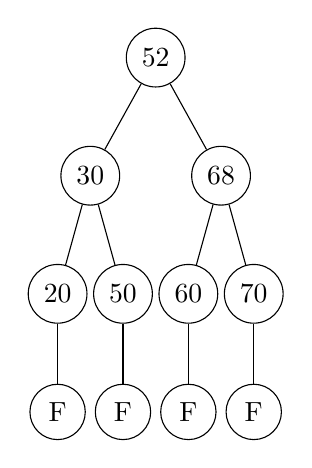
\begin{tikzpicture}
        \tikzset{every tree node/.style={minimum width=2em,draw,circle},
          blank/.style={draw=none},
          edge from parent/.style=
          {draw,edge from parent path={(\tikzparentnode) -- (\tikzchildnode)}},
          level distance=1.5cm}
          \Tree [.52
                  [.30
                    [.20 F ]
                    [.50 F ]]
                  [.68
                    [.60 F ]
                    [.70 F ]]]
      \end{tikzpicture} \\
      删去50: \\
      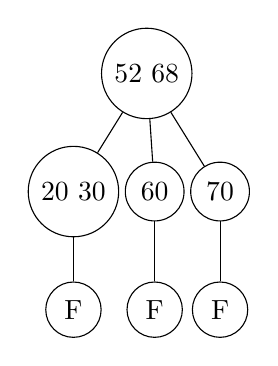
\begin{tikzpicture}
        \tikzset{every tree node/.style={minimum width=2em,draw,circle},
          blank/.style={draw=none},
          edge from parent/.style=
          {draw,edge from parent path={(\tikzparentnode) -- (\tikzchildnode)}},
          level distance=1.5cm}
          \Tree [.52\ 68
                  [.20\ 30 F ]
                  [.60 F ]
                  [.70 F ]]
      \end{tikzpicture} \\
      删去68: \\
      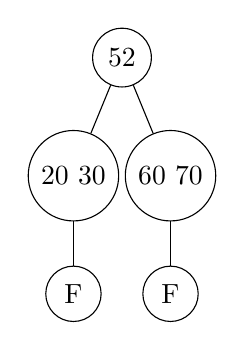
\begin{tikzpicture}
        \tikzset{every tree node/.style={minimum width=2em,draw,circle},
          blank/.style={draw=none},
          edge from parent/.style=
          {draw,edge from parent path={(\tikzparentnode) -- (\tikzchildnode)}},
          level distance=1.5cm}
          \Tree [.52
                  [.20\ 30 F ]
                  [.60\ 70 F ]]
      \end{tikzpicture} \\
    \end{solution}

  \item[9.] 习题9-19 \\
    \begin{solution}
      平均长度为:
      $$\frac{1}{8}(1+1+1+1+2+2+6+3)=\frac{17}{8}$$
    \end{solution}

  \item[10.] 习题9-24

  \item[11.] 习题10-1
    \begin{enumerate}
      \item [1)]
        (087,503,061,512,170,897,275,653,426,908) \\
        (087,061,503,170,512,275,653,426,897,908) \\
        (061,087,170,503,275,512,426,653,897,908) \\
        (061,087,170,275,426,503,512,653,897,908)
      \item [2)]
        (170,087,275,049,426,503,897,512,653,908) \\
        (170,049,275,087,426,503,653,512,897,908) \\
        (049,087,170,275,426,503,512,653,897,908)
      \item [3)]
        (087,061,170,275,426)(503)(512,908,897,653) \\
        (061)(087)(170,275,426)(503)(512)(908,897,653) \\
        (061)(087)(170)(275,426)(503)(512)(897,653)(908) \\
        (061)(087)(170)(275)(426)(503)(512)(653)(897)(908) \\
        (061,087,170,275,426,503,512,653,897,908)
      \item [5)]
        (503)(087)(512)(061)(908)(170)(897)(275)(653)(426) \\
        (503)(087)(512)(061,908)(170)(897)(275)(426,653) \\
        (087,503)(061,512,908)(170,897)(275,426,653) \\
        (061,087,503,512,908)(170,275,426,653,897) \\
        (061,087,170,275,426,503,512,653,897,908)
    \end{enumerate}

  \item[12.] 习题10-3 \\
    \begin{solution}
      堆排序、快速排序、希尔排序是不稳定的排序算法,而基数排序、插入排序、归并排序是稳定的排序算法。 \\
      希尔排序:2,2,1,3 \\
      快速排序:2,1,1,3 \\
    \end{solution}

  \item[13.] 习题10-15

  \item[14.] 习题10-21

  \item[15.] 习题11-1

  \item[16.] 习题11-2

  \item[17.] 习题11-5

  \item[18.] 习题11-11
\end{enumerate}
\end{document}
